% Paper v3: Ground-up refinement of style, deductive logic, and visual hierarchy.
% Build: pdflatex main.tex && bibtex main && pdflatex main.tex && pdflatex main.tex
\ifdefined\pdftexversion\pdfoutput=1\fi
\documentclass[11pt]{article}

\usepackage[utf8]{inputenc}
\usepackage[T1]{fontenc}
\usepackage[letterpaper, margin=1in]{geometry}
\usepackage{amsmath, amssymb, amsfonts, amsthm, mathtools}
\usepackage{graphicx}
\usepackage{booktabs}
\usepackage{multirow}
\usepackage{array}
\usepackage{enumitem}
\usepackage{microtype}
\usepackage{nicefrac}
\usepackage{pifont}
\usepackage[table]{xcolor}
\usepackage[round]{natbib}
\PassOptionsToPackage{hyphens}{url}
\usepackage{xurl}
\usepackage{paperstyle}

\pagestyle{paper}
\papershorttitle{Where Output-Cotangent Preconditioning Matters in Muon-Type Optimizers}
\graphicspath{{figs/}}
\urlstyle{tt}
\interfootnotelinepenalty=10000

\renewcommand{\topfraction}{0.90}
\renewcommand{\bottomfraction}{0.80}
\renewcommand{\textfraction}{0.08}
\renewcommand{\floatpagefraction}{0.80}

% Mathematical notation macros
\newcommand{\Tr}{{\mathsf{T}}}
\newcommand{\Nten}{\mathcal{N}_{10}}
\newcommand{\unitrms}{\operatorname{unitRMS}}
\newcommand{\tr}{\operatorname{tr}}
\newcommand{\Diag}{\operatorname{Diag}}
\newcommand{\diag}{\operatorname{diag}}
\newcommand{\E}{\mathbb{E}}
\newcommand{\R}{\mathbb{R}}
\newcommand{\dm}{d_{\mathrm{model}}}
\newcommand{\dff}{d_{\mathrm{ff}}}
\newcommand{\Lsel}{\mathcal{L}_{\mathrm{sel}}}
\newcommand{\Lc}{\mathcal{L}_{\mathrm{C4}}}
\newcommand{\Lpal}{\mathcal{L}_{\mathrm{Paloma}}}

% Consistent method names
\newcommand{\mname}[1]{#1}
\definecolor{colWT}{HTML}{1B4F9C}
\definecolor{colOD}{HTML}{0E7C7B}
\definecolor{colNull}{HTML}{C87D20}
\definecolor{colBad}{HTML}{C0392B}
\definecolor{rowtint}{HTML}{F2F6FC}

\newcommand{\cmark}{\textcolor{colOD}{\ding{51}}}
\newcommand{\xmark}{\textcolor{colBad}{\ding{55}}}

\title{Where Output-Cotangent Preconditioning Matters in Muon-Type Optimizers: Width-Thresholded Geometry and Asynchronous Execution}
\author{Optimizer Research Team}
\paperaffiliations{Preprint $\cdot$ Complete Reproducibility Archive: 168 Executed Training \& Benchmark Runs on $8\text{--}32\times\text{A100}$}

\begin{document}

\maketitle

\begin{abstract}
Orthogonalized-momentum optimizers (\mname{Muon}) benefit substantially from preconditioning on layer \emph{input} activation second moments (\mname{MuonT}), raising a foundational question: since a linear layer's weight gradient is $G = \sum \delta x^{\Tr}$, does preconditioning on \emph{output-cotangent} second moments $B = \E[\delta\delta^{\Tr}]$ provide complementary geometric signal in Transformer pretraining?
Auditing all 11 input and output second moments across a 32-layer Transformer along unpreconditioned \mname{Muon}, input-whitened \mname{MuonT}, and active two-sided \mname{WT-MLP-Lag} trajectories reveals a sharp, optimizer-invariant role- and width-dependent dichotomy.
Pre-SwiGLU MLP expansion outputs (\texttt{gate}, \texttt{up}, width $\dff = 4\dm$) concentrate $>91\%$ of their Frobenius energy and $78\%\text{--}91\%$ of their departure-from-identity anisotropy on the coordinate diagonal while consuming $96.2\%$ of dense $O(d^3)$ output eigendecomposition FLOPs; conversely, hidden-width outputs (\texttt{q}, \texttt{k}, \texttt{v}, \texttt{o}, \texttt{down}, width $\dm$)---especially residual-stream writers (\texttt{o}, \texttt{down}, $\le 1.0\%$ diagonal anisotropy)---are overwhelmingly rotational and drift up to $16\times$--$32\times$ faster in subspace than forward activations, triggering $3{,}714\times$ more post-warmup exact-eigendecomposition fallbacks along \mname{MuonT}.
Guided by these two empirical laws, we propose \mname{WT-MLP-Lag}, which pairs dense \mname{MuonT} input whitening with \emph{width-thresholded} output preconditioning---dense spectral inverse roots $(-1/2,\,-1/8)$ at width $\dm$ and exact per-step diagonal scaling at width $\dff$---and hides critical-path cotangent reduction and root tracking behind the next step via a one-update asynchronous lag, grouped Triton backward capture, chunked row-buffer reuse, and non-blocking batched fallback eigendecompositions, reducing two-sided step-time overhead from $+39\%$ to $+6.8\%\text{--}8.2\%$ over \mname{Muon} across \texttt{130M} and \texttt{520M}, of which only $+3.3\%\text{--}5.3\%$ sits above input-only \mname{MuonT}.
Across 168 archived runs (133 complete trainings and 35 matched timing benchmarks), matched execution-path null controls ($|\Delta\Lsel| = 0.0003$ nats) and full-budget learning-rate sweeps isolate genuine geometric improvements: against \mname{Muon}, \mname{WT-MLP-Lag} recovers $-0.0153$ held-out nats on all $3/3$ fresh post-selection seeds at \texttt{130M} ($2.68\text{B}$ tokens), $-0.0142$ held-out and $-0.0168$ 16-domain Paloma nats under $4\times$ Chinchilla overtraining ($80$ tokens/parameter, $10.74\text{B}$ tokens, $16/16$ domains won), and $-0.0093$ held-out and $-0.0089$ Paloma nats zero-shot at \texttt{520M} ($10.74\text{B}$ tokens, $15/16$ domains won)---adding a further $28\%$, $38\%$, and $43\%$ on top of what input-only \mname{MuonT} itself recovers, and beating tuned \mname{MuonT} directly by $-0.0034$, $-0.0040$, and $-0.0028$ nats. Purely diagonal output preconditioning (\mname{OD-All}) instead falls back onto \mname{MuonT} at \texttt{520M} while costing more than it.
Counterfactual direction diagnostics verify that output factors act via $17^\circ$--$23^\circ$ subspace rotation rather than implicit step-size inflation ($-1.5\%$ direction norm), outperforming recent curvature-aware polar methods (\mname{GO-MUON}, \mname{Mousse}) at fixed token budgets while delineating the exact quality--wall-clock Pareto frontier.
\end{abstract}

\section{Introduction}
\label{sec:intro}

Output preconditioning can improve a Muon optimizer that already whitens its inputs. The useful approximation depends on the projection: large MLP expansion outputs admit cheap coordinate scaling, while smaller residual-stream outputs benefit from dense factors that capture cross-channel structure. This distinction makes the second side practical. All-diagonal output factors (OD-All) give little or no held-out gain at 130M and fall behind MuonT when model width doubles, consistent with this distinction.

Muon maps matrix momentum toward a semi-orthogonal update using Newton--Schulz iterations~\citep{jordan2024muon}. MuonT, also called Toner, adds input activation moments around this map and improves pretraining loss~\citep{mohamadi2026toner}. For a linear layer $y=Wx$, however, the gradient $G=\sum_j\delta_jx_j^{\Tr}$ depends on both the forward activation $x_j$ and the output cotangent $\delta_j=\partial\ell/\partial y_j$. Input-only whitening uses one of these two signals. We ask whether the second moment of $\delta$ provides an additional benefit after input whitening, and what it costs to use it.

A symmetric formula does not imply symmetric computational needs. In the Transformers we study, the two expanded MLP outputs account for 96.2\% of nominal output eigendecomposition work, yet most of their anisotropy is diagonal. The outputs that write back into the residual stream are much smaller, but their unequal eigenvalues are almost invisible in coordinate second moments. Dense input factors remain useful even at expansion width. Output factors also arrive later in the step and require frequent eigenbasis repairs, making their scheduling a separate problem from input preconditioning.

\begin{figure}[t]
  \centering
  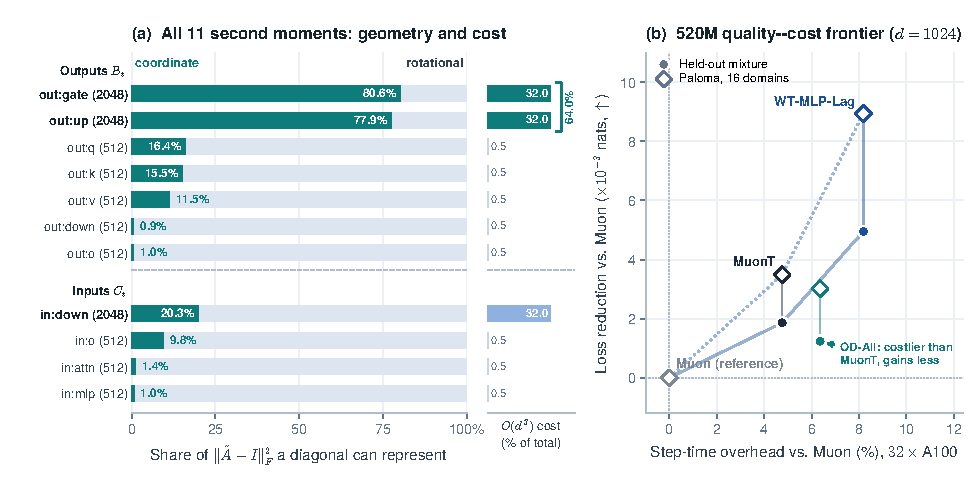
\includegraphics[width=\textwidth]{fig1_overview.pdf}
  \caption{\textbf{Output geometry suggests where dense preconditioning is worth its cost.}
  \textbf{(a)} Diagonal and off-diagonal shares of anisotropy for all 11 moments (130M, Muon trajectory, step 2,500). Each bar shows the 32-layer median of $\mathrm{DiagAniso}$ from \cref{eq:diag_aniso} and its complement, $1-\mathrm{DiagAniso}$. The split describes where anisotropy lies in the model's coordinate basis; it does not show its total magnitude. The cost column gives each moment's share of nominal dense eigendecomposition work across all 11 moments; teal marks the two moments WT-MLP-Lag diagonalizes. Expanded outputs have mostly diagonal anisotropy and account for 96.2\% of output-side cubic work; the equally wide \texttt{down} input retains cross-channel structure.
  \textbf{(b)} Final held-out and Paloma gains versus Muon at 520M, against median step-time overhead on 32 A100 GPUs. WT-MLP-Lag extends MuonT's quality gain with an incremental throughput cost. This run uses one seed.}
 \label{fig:overview}
\end{figure}

We build \mname{WT-MLP-Lag} around these observations. It retains MuonT's dense input factors, uses dense output factors at hidden width, and uses diagonal output factors on the expanded \texttt{gate} and \texttt{up} projections. A one-update lag lets the output reduction and root solver overlap the next training step. The mathematical approximation removes most of the nominal cubic output work; asynchronous execution reduces the exposed latency that remains.

The resulting gains survive three tests: fresh paired seeds at 130M, four times as many training tokens, and transfer to 520M without retuning the output-side recipe (\Cref{fig:scaling_traj}). Matched-path identity controls and full-budget learning-rate sweeps reduce two sources of misleading optimizer comparisons. Counterfactual updates then test how the method changes the direction and norm of the step. Together these experiments support a practical design rule: preserve dense output geometry where channel correlations dominate, and approximate it where coordinate energy carries most of the signal.

Our evidence covers models up to 537M non-embedding parameters. It establishes a fixed-token quality improvement; the systems measurements retain a throughput penalty, and the longer and wider training comparisons still need multi-seed replication.

\section{Structural Diagnosis: Where Does Output Geometry Live?}
\label{sec:diagnosis}

Before designing an output-side preconditioner, we ask an empirical question across unpreconditioned, input-whitened, and two-sided preconditioned training: \emph{what is the actual covariance and temporal structure of every input activation and output cotangent in a Transformer, and does active preconditioning alter that geometry?}
Auditing three matched trajectories---\mname{Muon}, \mname{MuonT}, and \mname{WT-MLP-Lag}---separates intrinsic architectural invariants of pre-RMSNorm SwiGLU Transformers from optimizer-induced adaptation.

\subsection{Preliminaries and Three-Trajectory Moment Audit}
\label{sec:diagnosis_setup}

Consider a 2D linear projection $y = W x$ with weight $W_t \in \R^{m \times n}$ at step $t$ (rows index output coordinates $m$; columns index input coordinates $n$).
In a Llama-style pre-RMSNorm Transformer block with hidden width $\dm$ and SwiGLU expansion width $\dff = 4\dm$, each layer $\ell \in \{1,\dots,L\}$ contains seven 2D projections:
four square attention matrices $W_q, W_k, W_v, W_o \in \R^{\dm \times \dm}$, two tall MLP expansion matrices $W_{\mathrm{gate}}, W_{\mathrm{up}} \in \R^{\dff \times \dm}$, and one wide MLP contraction matrix $W_{\mathrm{down}} \in \R^{\dm \times \dff}$.

\paragraph{Input vs.\ output second moments.}
During forward and backward propagation over $N_t$ sampled token positions pooled globally across ranks and microbatches ($286$ positions per $4{,}096$-token sequence, $N_t = 36{,}608$ per $0.5\text{M}$-token batch), each projection observes activations $x_{p,t,j} \in \R^{n_p}$ and unaveraged summed-loss output cotangents $\delta_{p,t,j} = \partial \sum \ell / \partial y_{p,t,j} \in \R^{m_p}$, yielding exponential moving averages (EMAs):
\begin{equation}
  C_{g(p),t} = \beta C_{g(p),t-1} + \frac{1-\beta}{N_t}\sum_{j=1}^{N_t} x_{p,t,j} x_{p,t,j}^{\Tr},
  \qquad
  B_{p,t} = \beta B_{p,t-1} + \frac{1-\beta}{N_t}\sum_{j=1}^{N_t} \delta_{p,t,j} \delta_{p,t,j}^{\Tr},
  \label{eq:moments}
\end{equation}
with $\beta = 0.938$ (effective averaging horizon $(1-\beta)^{-1} \approx 16.1$ updates).
Crucially, sharing differs between the two sides: because $W_q, W_k, W_v$ consume identical post-RMSNorm activations and $W_{\mathrm{gate}}, W_{\mathrm{up}}$ consume identical MLP post-RMSNorm activations, there are only 4 input moments per layer (\texttt{in:attn}, \texttt{in:o}, \texttt{in:mlp} at width $\dm$; \texttt{in:down} at width $\dff$).
On the output side, however, every projection receives a distinct backpropagated cotangent---even \texttt{out:o} and \texttt{out:down} write to sequential residual nodes separated by the MLP---requiring 7 separate output moments per layer ($5$ at width $\dm$ and $2$ at width $\dff$, or $224$ matrices across $L=32$ layers).

\paragraph{Trace-normalized inverse roots, three trajectories, and three diagnostic metrics.}
Following \mname{MuonT}~\citep{mohamadi2026toner}, any positive-trace symmetric moment $F \in \R^{d \times d}$ is trace-normalized and damped via
\begin{equation}
  A_d(F) = \frac{d\,F}{\tr(F)} + \epsilon I_d, \qquad \epsilon = 10^{-3},
  \label{eq:trace_norm}
\end{equation}
so that an isotropic moment satisfies $A_d(\alpha I_d) = (1+\epsilon)I_d$ and any constant positive cotangent scaling cancels identically.
From $A_d(F)$, \mname{MuonT} forms split inner and unit-RMS outer inverse roots $\mathsf{In}_d(F) = A_d(F)^{-1/2}$ and $\mathsf{Out}_d(F) = \sqrt{d}\,A_d(F)^{-1/8} / \|A_d(F)^{-1/8}\|_F$.

To audit all $11 \times 32 = 352$ full $d \times d$ FP32 moments at matched \texttt{130M} ($\dm=512, \dff=2048$, \texttt{seed 0}, $0.5\text{M}$ batch), we examine three trajectories:
(i) \mname{Muon} ($\eta=0.016$), via an exact $500$-step passive moment replay from the saved step-$2{,}000$ checkpoint through steps $2{,}250$ and $2{,}500$ ($0.0$ loss and weight divergence; $\beta^{250} = 1.1\times 10^{-7}$ and $\beta^{500} = 1.3\times 10^{-14}$ residual initialization weight);
(ii) \mname{MuonT} ($\eta=0.02263$, recorded via \mname{Null-Dense} across $10$ checkpoints over all $5{,}120$ steps while applying $L=\hat{L}=I$); and
(iii) \mname{WT-MLP-Lag} ($\eta=0.02263$, abbreviated \mname{WT} in \Cref{tab:diagnosis}), via a $500$-step \texttt{fast\_lag} replay through steps $2{,}250$ and $2{,}500$ that records all nine active dense groups alongside passive $2{,}048\times 2{,}048$ \texttt{out:gate,up} moments (matching active 1D diagonal accumulators to $\le 4.0\times 10^{-5}$ relative $\ell_2$ error across all 8 ranks; see \Cref{app:appendix_mech}).
On $\tilde{A} = d\,F/\tr(F)$ (unit mean diagonal $\frac{1}{d}\tr(\tilde{A}) = 1$), we evaluate:
\begin{enumerate}[leftmargin=1.6em, itemsep=2pt, topsep=3pt]
  \item \textbf{Pythagorean diagonal anisotropy share:}
  Because $\|\tilde{A} - I_d\|_F^2 = \|\diag(\tilde{A}) - \mathbf{1}\|_2^2 + \|\tilde{A} - \Diag(\tilde{A})\|_F^2$ holds to machine precision,
  \begin{equation}
    \mathrm{DiagAniso}(F) \triangleq \frac{\|\diag(\tilde{A}) - \mathbf{1}\|_2^2}{\|\tilde{A} - I_d\|_F^2} \in [0, 1]
    \label{eq:diag_aniso}
  \end{equation}
  measures the exact fraction of total departure-from-isotropy variance carried by per-coordinate scale differences rather than off-diagonal cross-coordinate correlations (quantified alongside the off-diagonal correlation RMS $\rho_{\mathrm{rms}} = \bigl[\frac{1}{d(d-1)}\sum_{i\neq j} F_{ij}^2/(F_{ii}F_{jj})\bigr]^{1/2}$).
  \item \textbf{Diagonal inverse-root explained variance:}
  Comparing the dense inner root $L = A_d(F)^{-1/2}$ to its elementwise diagonal counterpart $L_{\diag} = \Diag(\tilde{A} + \epsilon I_d)^{-1/2}$,
  \begin{equation}
    R^2(A_d^{-1/2}) \triangleq 1 - \frac{\|L - L_{\diag}\|_F^2}{\|L - I_d\|_F^2}
    \label{eq:r2_root}
  \end{equation}
  measures how much of the dense whitening operator's nontrivial action is captured by O($d$) coordinate scaling alone.
  \item \textbf{Subspace Grassmann drift:}
  Letting $V_{k,t} \in \R^{d \times k}$ denote the top-$k$ eigenvectors of $F_t$, $\mathrm{Drift}_{16}(t) \triangleq 1 - \frac{1}{16}\|V_{16,t}^{\Tr}V_{16,t-250}\|_F^2 = \frac{1}{32}\|V_{16,t}V_{16,t}^{\Tr} - V_{16,t-250}V_{16,t-250}^{\Tr}\|_F^2 \in [0,1]$ measures how rapidly the dominant 16-dimensional eigenspace rotates over $250$ updates.
\end{enumerate}

\begin{table}[t]
  \centering
  \caption{\textbf{Three-trajectory structural and temporal audit across all 11 Transformer second moments} (\texttt{130M}, $352$ FP32 EMA matrices across $L=32$ layers) comparing unpreconditioned \mname{Muon}, input-whitened \mname{MuonT}, and active two-sided \mname{WT-MLP-Lag} (\mname{WT}). Metric groups 1--5 report step-$2{,}500$ ($1.31\text{B}$-token) 32-layer medians; $\mathrm{Drift}_{16}$ reports the 32-layer mean over steps $2{,}250 \to 2{,}500$. Across all three trajectories, pre-SwiGLU expansion outputs (\texttt{out:gate}, \texttt{out:up}) hug the $0.0052$ sampling floor with $78\%\text{--}91\%$ diagonal anisotropy ($R^2 = 76\%\text{--}99\%$), whereas residual-stream outputs (\texttt{out:o}, \texttt{out:down}) remain $\ge 99\%$ rotational ($\mathrm{DiagAniso} = 0.8\%\text{--}1.0\%$).}
  \label{tab:diagnosis}
  \vspace{2pt}
  \footnotesize\setlength{\tabcolsep}{2.3pt}%
  \resizebox{\textwidth}{!}{%
  \begin{tabular}{@{}l@{\hspace{6pt}}r@{\hspace{9pt}}rrr@{\hspace{9pt}}rrr@{\hspace{9pt}}rrr@{\hspace{9pt}}rrr@{\hspace{9pt}}rrr@{\hspace{9pt}}rrr@{}}
    \toprule
    & & \multicolumn{3}{c@{\hspace{9pt}}}{$\mathrm{erank}/d$ (\%)} & \multicolumn{3}{c@{\hspace{9pt}}}{$\mathrm{CV}_{\diag}$} & \multicolumn{3}{c@{\hspace{9pt}}}{$\rho_{\mathrm{rms}}$} & \multicolumn{3}{c@{\hspace{9pt}}}{$\mathrm{DiagAniso}$ (\%)} & \multicolumn{3}{c@{\hspace{9pt}}}{$R^2(A_d^{-1/2})$ (\%)} & \multicolumn{3}{c@{}}{$\mathrm{Drift}_{16}$} \\
    \cmidrule(r{9pt}){3-5}\cmidrule(r{9pt}){6-8}\cmidrule(r{9pt}){9-11}\cmidrule(r{9pt}){12-14}\cmidrule(r{9pt}){15-17}\cmidrule{18-20}
    Moment Group & $d$ & \multicolumn{1}{c}{\tiny\mname{Muon}} & \multicolumn{1}{c}{\tiny\mname{MuonT}} & \multicolumn{1}{c@{\hspace{9pt}}}{\tiny\mname{WT}} & \multicolumn{1}{c}{\tiny\mname{Muon}} & \multicolumn{1}{c}{\tiny\mname{MuonT}} & \multicolumn{1}{c@{\hspace{9pt}}}{\tiny\mname{WT}} & \multicolumn{1}{c}{\tiny\mname{Muon}} & \multicolumn{1}{c}{\tiny\mname{MuonT}} & \multicolumn{1}{c@{\hspace{9pt}}}{\tiny\mname{WT}} & \multicolumn{1}{c}{\tiny\mname{Muon}} & \multicolumn{1}{c}{\tiny\mname{MuonT}} & \multicolumn{1}{c@{\hspace{9pt}}}{\tiny\mname{WT}} & \multicolumn{1}{c}{\tiny\mname{Muon}} & \multicolumn{1}{c}{\tiny\mname{MuonT}} & \multicolumn{1}{c@{\hspace{9pt}}}{\tiny\mname{WT}} & \multicolumn{1}{c}{\tiny\mname{Muon}} & \multicolumn{1}{c}{\tiny\mname{MuonT}} & \multicolumn{1}{c@{}}{\tiny\mname{WT}} \\
    \midrule
    \multicolumn{20}{@{}l}{\emph{Right-input second moments $C_t = \E[x x^{\Tr}]$ (4 per layer, 128 total)}} \\
    \texttt{in:attn} ($q,k,v$)       & 512  & $30.0$ & $17.9$ & $18.0$ & $0.63$ & $0.84$ & $0.76$ & $0.1465$ & $0.2031$ & $0.2066$ & $1.4$ & $1.0$ & $0.8$ & $8.2$ & $10.6$ & $10.1$ & $0.041$ & $0.021$ & $0.023$ \\
    \texttt{in:o}                    & 512  & $37.9$ & $20.8$ & $23.4$ & $0.77$ & $0.75$ & $0.77$ & $0.0968$ & $0.2120$ & $0.2001$ & $9.8$ & $1.8$ & $1.8$ & $30.1$ & $22.5$ & $26.5$ & $0.107$ & $0.094$ & $0.108$ \\
    \texttt{in:mlp} ($\text{gate,up}$) & 512 & $33.8$ & $21.6$ & $19.5$ & $0.48$ & $0.64$ & $0.62$ & $0.1410$ & $0.1959$ & $0.2024$ & $1.0$ & $0.8$ & $0.7$ & $4.9$ & $6.0$ & $6.7$ & $0.046$ & $0.021$ & $0.025$ \\
    \texttt{in:down} (post-SwiGLU)   & 2048 & $67.1$ & $29.1$ & $35.6$ & $0.71$ & $2.92$ & $2.33$ & $0.0283$ & $0.0346$ & $0.0359$ & $20.3$ & $43.4$ & $34.7$ & $91.3$ & $79.4$ & $78.7$ & $0.186$ & $0.106$ & $0.087$ \\
    \addlinespace[2.5pt]
    \multicolumn{20}{@{}l}{\emph{Left-cotangent second moments $B_t = \E[\delta \delta^{\Tr}]$ (7 per layer, 224 total)}} \\
    \texttt{out:q}                   & 512  & $38.5$ & $38.5$ & $29.3$ & $1.04$ & $0.97$ & $1.14$ & $0.0615$ & $0.0641$ & $0.0732$ & $16.4$ & $18.0$ & $13.3$ & $64.8$ & $62.4$ & $66.0$ & $0.150$ & $0.140$ & $0.110$ \\
    \texttt{out:k}                   & 512  & $24.4$ & $23.7$ & $13.0$ & $1.45$ & $1.50$ & $1.87$ & $0.0746$ & $0.0774$ & $0.0779$ & $15.5$ & $14.4$ & $14.7$ & $77.6$ & $71.8$ & $78.6$ & $0.178$ & $0.165$ & $0.147$ \\
    \texttt{out:v}                   & 512  & $47.0$ & $50.4$ & $41.5$ & $0.63$ & $0.58$ & $0.57$ & $0.0600$ & $0.0560$ & $0.0749$ & $11.5$ & $12.2$ & $6.8$ & $38.6$ & $31.2$ & $19.9$ & $0.664$ & $0.662$ & $0.586$ \\
    \textcolor{colWT}{\textbf{\texttt{out:o} (residual)}}    & \textcolor{colWT}{\textbf{512}} & $83.3$ & $85.3$ & $78.2$ & $0.09$ & $0.06$ & $0.10$ & $0.0307$ & $0.0301$ & $0.0393$ & \textcolor{colWT}{$\mathbf{1.0}$} & \textcolor{colWT}{$\mathbf{0.8}$} & \textcolor{colWT}{$\mathbf{0.8}$} & \textcolor{colWT}{$\mathbf{3.6}$} & \textcolor{colWT}{$\mathbf{1.2}$} & \textcolor{colWT}{$\mathbf{2.3}$} & $0.164$ & $0.134$ & $0.103$ \\
    \textcolor{colWT}{\textbf{\texttt{out:down} (residual)}} & \textcolor{colWT}{\textbf{512}} & $84.3$ & $84.6$ & $77.9$ & $0.08$ & $0.07$ & $0.09$ & $0.0315$ & $0.0312$ & $0.0403$ & \textcolor{colWT}{$\mathbf{0.9}$} & \textcolor{colWT}{$\mathbf{0.8}$} & \textcolor{colWT}{$\mathbf{0.8}$} & \textcolor{colWT}{$\mathbf{2.3}$} & \textcolor{colWT}{$\mathbf{1.2}$} & \textcolor{colWT}{$\mathbf{1.4}$} & $0.123$ & $0.107$ & $0.072$ \\
    \rowcolor{rowtint}
    \textcolor{colOD}{\textbf{\texttt{out:gate} (pre-SwiGLU)}} & \textcolor{colOD}{\textbf{2048}} & $88.2$ & $87.1$ & $72.8$ & $0.55$ & $0.59$ & $1.32$ & \textcolor{colOD}{$\mathbf{0.0055}$} & \textcolor{colOD}{$\mathbf{0.0051}$} & \textcolor{colOD}{$\mathbf{0.0048}$} & \textcolor{colOD}{$\mathbf{80.6}$} & \textcolor{colOD}{$\mathbf{82.0}$} & \textcolor{colOD}{$\mathbf{89.5}$} & \textcolor{colOD}{$\mathbf{98.8}$} & \textcolor{colOD}{$\mathbf{82.2}$} & \textcolor{colOD}{$\mathbf{94.9}$} & $0.292$ & $0.240$ & $0.159$ \\
    \rowcolor{rowtint}
    \textcolor{colOD}{\textbf{\texttt{out:up} (pre-SwiGLU)}}   & \textcolor{colOD}{\textbf{2048}} & $83.8$ & $82.5$ & $47.3$ & $0.68$ & $0.75$ & $2.83$ & \textcolor{colOD}{$\mathbf{0.0068}$} & \textcolor{colOD}{$\mathbf{0.0073}$} & \textcolor{colOD}{$\mathbf{0.0082}$} & \textcolor{colOD}{$\mathbf{77.9}$} & \textcolor{colOD}{$\mathbf{78.1}$} & \textcolor{colOD}{$\mathbf{90.8}$} & \textcolor{colOD}{$\mathbf{98.2}$} & \textcolor{colOD}{$\mathbf{75.9}$} & \textcolor{colOD}{$\mathbf{91.9}$} & $0.251$ & $0.215$ & $0.130$ \\
    \bottomrule
  \end{tabular}%
  }
\end{table}

\subsection{Finding 1: The Width-and-Role Dichotomy Across Output Moments}
\label{sec:dichotomy}

\Cref{tab:diagnosis} and \Cref{fig:structural_audit}a reveal that output cotangent moments partition sharply into three architectural regimes governed by projection width and nonlinearity placement---a dichotomy that holds across unpreconditioned \mname{Muon}, input-whitened \mname{MuonT}, and active two-sided \mname{WT-MLP-Lag} (as well as full dense \mname{DT-All}; \Cref{app:appendix_mech}):

\paragraph{1. Expanded pre-SwiGLU outputs (\texttt{out:gate}, \texttt{out:up}; $d = \dff$) are coordinate-dominated across all three optimizers.}
Because SwiGLU computes $z = \operatorname{SiLU}(y_{\mathrm{gate}}) \odot y_{\mathrm{up}}$ elementwise across the $\dff$ intermediate channels, backpropagating through the elementwise gate multiplies each coordinate by a weakly correlated gate factor, driving cross-channel correlations toward zero while compounding coordinate variance spread.
Across \mname{Muon} / \mname{MuonT} / \mname{WT-MLP-Lag}, \texttt{out:gate} and \texttt{out:up} concentrate $94.9\% / 94.9\% / 94.1\%$ and $91.9\% / 91.2\% / 92.4\%$ of their raw Frobenius energy and $80.6\% / 82.0\% / 89.5\%$ and $77.9\% / 78.1\% / 90.8\%$ of their centered anisotropy ($\mathrm{DiagAniso}$) on the diagonal, while their off-diagonal correlation RMS ($\rho_{\mathrm{rms}} = 0.0055 / 0.0051 / 0.0048$ and $0.0068 / 0.0073 / 0.0082$) sits directly at the finite-sample floor $1/\sqrt{N_t} = 0.0052$!
Consequently, an $O(\dff)$ diagonal inverse root explains $98.8\% / 82.2\% / 94.9\%$ and $98.2\% / 75.9\% / 91.9\%$ of dense $A_d(B)^{-1/2}$ across all 32 layers ($\cos(L, L_{\diag}) = 0.996\text{--}0.998$ on \texttt{gate} and $0.993\text{--}0.997$ on \texttt{up}): active inline diagonal normalization under \mname{WT-MLP-Lag} induces zero off-diagonal coupling while deepening per-neuron scale specialization ($\mathrm{CV}_{\diag}$ rising from $0.55 / 0.59$ to $1.32$ on \texttt{gate} and from $0.68 / 0.75$ to $2.83$ on \texttt{up}).

\paragraph{2. Residual-stream writers (\texttt{out:o}, \texttt{out:down}; $d = \dm$) are $\ge 99\%$ rotational on every trajectory.}
At the opposite extreme, projections writing directly into the shared residual stream exhibit uniform per-coordinate cotangent variance under every optimizer ($\mathrm{CV}_{\diag} = 0.09 / 0.06 / 0.10$ on \texttt{out:o} and $0.08 / 0.07 / 0.09$ on \texttt{out:down}).
As a result, $\mathrm{DiagAniso}$ collapses to $0.8\%\text{--}1.0\%$, and diagonal inverse roots capture only $1.2\%\text{--}3.6\%$ of $A_d(B)^{-1/2}$ ($R^2 \le 2.5\%$ across \mname{MuonT}'s entire 8-checkpoint trajectory)!
Yet $B_o$ and $B_{\mathrm{down}}$ are far from isotropic (mean top-to-mean eigenvalue ratios $42.4$ and $40.5$ on \mname{MuonT}), making any purely diagonal output preconditioner (\mname{OD-All}) nearly an identity map on $W_o$ and $W_{\mathrm{down}}$.

\paragraph{3. Attention internal outputs (\texttt{out:q,k,v}; $d = \dm$) and post-SwiGLU inputs (\texttt{in:down}; $d = \dff$) are mixed.}
Within attention, \texttt{out:q} and \texttt{out:k} combine head-level scale variation with rotary/attention-score coupling ($R^2 = 62.4\%\text{--}66.0\%$ and $71.8\%\text{--}78.6\%$), while \texttt{out:v} remains predominantly rotational ($\mathrm{DiagAniso} = 6.8\%\text{--}12.2\%, R^2 = 19.9\%\text{--}38.6\%$).
On the input side, RMSNormed \texttt{in:attn} and \texttt{in:mlp} are $98.6\%$--$99.3\%$ rotational across all three runs ($\mathrm{DiagAniso} = 0.7\%$--$1.4\%$; active input whitening sharpens \texttt{in:attn} $\mathrm{erank}/d$ from $30.0\%$ on \mname{Muon} to $17.9\% / 18.0\%$ on \mname{MuonT} / \mname{WT}), whereas post-SwiGLU \texttt{in:down} retains $79.7\%$, $56.6\%$, and $65.3\%$ off-diagonal moment anisotropy across \mname{Muon}, \mname{MuonT}, and \mname{WT-MLP-Lag} ($\rho_{\mathrm{rms}} = 0.0283 / 0.0346 / 0.0359$, $5.1\times$--$7.5\times$ above \texttt{out:gate}) alongside large coordinate skew ($R^2 = 91.3\% / 79.4\% / 78.7\%$).

\begin{figure}[t]
  \centering
  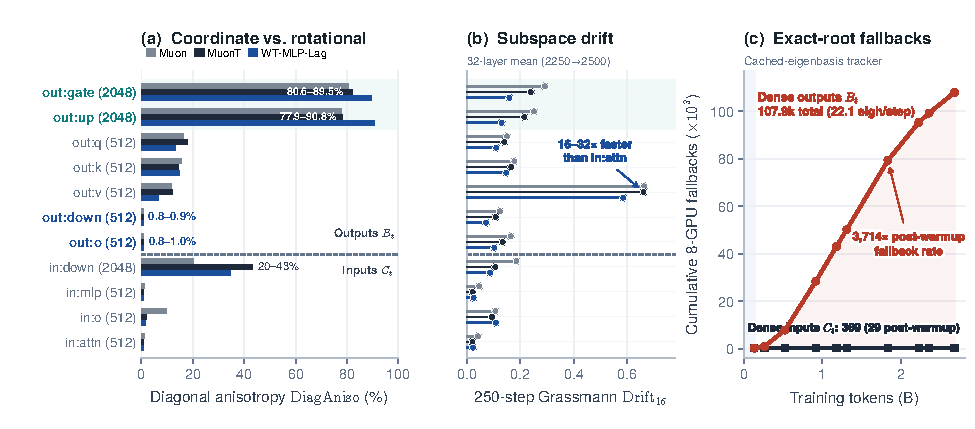
\includegraphics[width=\textwidth]{fig2_structural_audit.pdf}
  \caption{\textbf{Three-trajectory structural and temporal anatomy of the 11 Transformer second moments (\texttt{130M}).}
  \textbf{(a)} Pythagorean diagonal anisotropy share ($\mathrm{DiagAniso}$) across \mname{Muon}, \mname{MuonT}, and \mname{WT-MLP-Lag} consistently separates coordinate-dominated $\dff=2048$ MLP outputs (\texttt{out:gate} $80.6\%$--$89.5\%$, \texttt{out:up} $77.9\%$--$90.8\%$) from rotation-dominated $\dm=512$ residual outputs (\texttt{out:o, down} $0.8\%$--$1.0\%$) and inputs.
  \textbf{(b)} Backward cotangent top-16 eigenspaces drift an order of magnitude faster over 250 steps than RMSNormed forward activations across all three trajectories ($16\times$--$32\times$ faster on \texttt{out:v} vs.\ \texttt{in:attn}).
  \textbf{(c)} Rapid subspace drift causes Toner's cached-eigenbasis root solver on \mname{Null-Dense} (\mname{MuonT}) to trigger $107{,}911$ exact eigendecomposition fallbacks on dense outputs ($22.1/\text{step}$) vs.\ only $369$ ($29$ post-warmup) on inputs.}
  \label{fig:structural_audit}
\end{figure}

\subsection{Finding 2: Cubic Cost Concentration and Subspace Non-Stationarity}
\label{sec:drift_cost}

Why does naive dense two-sided preconditioning (\mname{DT-All}) incur a prohibitive $+39.2\%$ step-time penalty?
Combining \Cref{tab:diagnosis} with systems counters (\Cref{fig:structural_audit}b,c) exposes two compounding bottlenecks:
\begin{enumerate}[leftmargin=1.6em, itemsep=2pt, topsep=3pt]
  \item \textbf{$96.2\%$ of dense output $O(d^3)$ work sits where off-diagonal signal vanishes.}
  Each layer tracks five $\dm$-wide and two $\dff = 4\dm$-wide output moments.
  Because dense eigendecomposition scales as $O(d^3)$ and Gram storage/communication scales as $O(d^2)$, the two $\dff$-wide matrices (\texttt{out:gate}, \texttt{out:up}) consume $\frac{2 \cdot 4^3}{2 \cdot 4^3 + 5 \cdot 1^3} = \frac{128}{133} = 96.24\%$ of dense output eigendecomposition FLOPs and $\frac{2 \cdot 4^2}{2 \cdot 4^2 + 5 \cdot 1^2} = 86.49\%$ of packed Gram bytes ($0.50\text{ GiB}$ of $0.58\text{ GiB}$ per rank)---precisely the two moments whose off-diagonal correlations lie at the sampling noise floor across every optimizer!
  \item \textbf{Rapid cotangent subspace drift breaks cached-eigenbasis root tracking.}
  Toner's fast root engine avoids computing exact eigendecompositions at every step by iterating in a cached eigenbasis refreshed asynchronously every $4$ steps, falling back to exact GPU \texttt{eigh} only when residual error exceeds tolerance~\citep{mohamadi2026toner}.
  Forward RMSNormed eigenspaces move slowly even on \mname{Muon} ($\mathrm{Drift}_{16} = 0.041,\,0.046$ on \texttt{in:attn, mlp}) and halve in drift under input whitening ($0.021,\,0.021$ on \mname{MuonT} and $0.023,\,0.025$ on \mname{WT-MLP-Lag}), producing only $29$ post-warmup fallbacks across all 8 GPUs over Steps $250\text{--}5{,}120$ ($0.006/\text{step}$).
  On backward cotangents, however, top-16 subspaces rotate far faster across all three trajectories: \texttt{out:up, gate} sit at $0.251,\,0.292$ (\mname{Muon}), $0.215,\,0.240$ (\mname{MuonT}, $10.4\times$--$11.6\times$ \texttt{in:attn}), and $0.130,\,0.159$ (\mname{WT-MLP-Lag}), while \texttt{out:v} reaches $\mathrm{Drift}_{16} = 0.664 / 0.662 / 0.586$ ($16.2\times$, $32\times$, and $25.8\times$ faster than \texttt{in:attn}; \Cref{fig:structural_audit}b).
  Consequently, dense output tracking triggers $107{,}701$ post-warmup exact fallbacks ($3{,}714\times$ more than inputs, or $22.1$ exact eigendecompositions every step; \Cref{fig:structural_audit}c)---all sitting on the post-backward critical path if awaited synchronously.
\end{enumerate}

\begin{takeaway}[Two Design Laws for Output-Cotangent Preconditioning]
(1) Width-Thresholded Factorization: Diagonalizing $\dff$-wide pre-SwiGLU cotangents (\texttt{gate, up}) eliminates $96.2\%$ of output $O(d^3)$ eigendecomposition work while retaining $76\%\text{--}99\%$ of dense root fidelity across \mname{Muon}, \mname{MuonT}, and \mname{WT-MLP-Lag} ($92\%\text{--}95\%$ under active \mname{WT-MLP-Lag}), whereas $\dm$-wide cotangents (\texttt{q, k, v, o, down}) must remain dense to capture rotational residual geometry.
(2) Asynchronous Execution: Because cotangents arrive after backward and drift up to $16\times$--$32\times$ faster than activations, dense $\dm$-wide output roots must be overlapped across step boundaries rather than awaited on the critical path.
\end{takeaway}

\section{Method: Width-Thresholded Geometry and Asynchronous Execution}
\label{sec:method}

Directly translating the two structural laws from \Cref{sec:diagnosis} into an optimizer and distributed runtime yields \mname{WT-MLP-Lag}.
We first specify the unified two-sided operator family and width-thresholded factorization (\Cref{sec:operator}), then detail the three-pillar systems co-design that hides critical-path cotangent latency across $8\text{--}32\times\text{A100}$ (\Cref{sec:systems}).

\subsection{Unified Two-Sided Operator Family and Width Thresholding}
\label{sec:operator}

For each 2D Transformer block projection $p \in \{\text{q, k, v, o, gate, up, down}\}$ of shape $m_p \times n_p$ with globally averaged gradient $G_{p,t} \in \R^{m_p \times n_p}$, we maintain standard Nesterov momentum without $(1-\mu)$ dampening:
\begin{equation}
  M_{p,t} = \mu M_{p,t-1} + G_{p,t}, \qquad U_{p,t} = G_{p,t} + \mu M_{p,t}, \qquad \mu = 0.95,\quad M_{p,-1} = 0.
  \label{eq:momentum}
\end{equation}
Let $\Nten:\R^{m \times n} \to \R^{m \times n}$ denote the executed 10-step quintic Newton--Schulz map with coefficients $(3.4445,\,-4.7750,\,2.0315)$, Frobenius normalization floor $10^{-5}$, and BF16-operand / FP32-accumulate GEMMs (\texttt{tpu} mode; exact specification in \Cref{app:appendix_math}).
Given right (input) inner/outer factors $(R_{p,t},\,\hat{R}_{p,t}) \in \R^{n_p \times n_p}$ built from $C_{g(p),t}$ and left (output) inner/outer factors $(L_{p,t-\tau},\,\hat{L}_{p,t-\tau}) \in \R^{m_p \times m_p}$ built from $B_{p,t-\tau}$ at lag $\tau \in \{0, 1\}$, every method in our study updates $W_{p,t}$ via
\begin{equation}
  D_{p,t} = \hat{L}_{p,t-\tau}\,\Nten\!\left(L_{p,t-\tau}\,U_{p,t}\,R_{p,t}\right)\hat{R}_{p,t},
  \qquad
  W_{p,t+1} = W_{p,t} - \eta_t\left(s_{m_p,n_p}\,D_{p,t} + \lambda\,Q_{p,t}\right),
  \label{eq:update}
\end{equation}
where $s_{m,n} = \sqrt{\max(1, m/n)}$ ($s=2$ for tall \texttt{gate, up}; $s=1$ otherwise), $\lambda = 0.1$ is the decoupled weight-decay coefficient, and $Q_{p,t} = W_{p,t}\hat{R}_{p,t}^2$ when right outer factors are active (falling back to $\hat{L}_{p,t-\tau}^2 W_{p,t}$ for left-only ablations and $W_{p,t}$ for \mname{Muon}).
Embeddings, the untied output head, and RMSNorm gains remain routed to auxiliary AdamW cleanly separated from \Cref{eq:update}.

\paragraph{Dense vs.\ diagonal factor operators and scale preservation.}
Each active factor slot in \Cref{eq:update} instantiates \Cref{eq:trace_norm} in either dense spectral form ($\mathsf{Dense}$) or elementwise diagonal form ($\mathsf{Diag}$, using $f = \diag(F)$ and $a = d\,f/(\mathbf{1}^{\Tr}f) + \epsilon\mathbf{1}$):
\begin{align}
  L^{\mathsf{Dense}} &= A_m(B)^{-1/2}, &
  \hat{L}^{\mathsf{Dense}} &= \unitrms\!\bigl(A_m(B)^{-1/8}\bigr), \label{eq:dense_roots}\\
  L^{\mathsf{Diag}} &= \Diag\!\bigl(a(B)^{-1/2}\bigr), &
  \hat{L}^{\mathsf{Diag}} &= \unitrms\!\bigl(\Diag(a(B)^{-1/8})\bigr), \label{eq:diag_roots}
\end{align}
where $\unitrms(X) \triangleq \sqrt{d}\,X / \|X\|_F$ enforces $\frac{1}{d}\|\unitrms(X)\|_F^2 = 1$ (with zero-trace startup moments returning $I_d$).
Two deliberate design choices distinguish \Cref{eq:update,eq:dense_roots,eq:diag_roots} from prior two-sided proposals:
\begin{enumerate}[leftmargin=1.6em, itemsep=2pt, topsep=2pt]
  \item \textbf{Decoupled $(-1/2,\,-1/8)$ powers with unit-RMS outer scaling (no global norm grafting).}
  Matching \mname{MuonT}'s input recipe, the unnormalized $-1/2$ inner factor whitens the singular frame \emph{entering} $\Nten$ (where $\Nten$'s initial Frobenius normalization absorbs global scale), while the gentler unit-RMS $-1/8$ outer factor reweights output coordinates \emph{after} $\Nten$ without inflating the update Frobenius norm ($\|D\|_F / \|D_{\text{MuonT}}\|_F = 0.985$; \Cref{sec:mechanism}).
  Consequently, \mname{MuonT}'s learning rate transfers directly without ad-hoc post-hoc Frobenius norm grafting.
  \item \textbf{Retaining input-shaped weight decay $Q_{p,t} = W_{p,t}\hat{R}_{p,t}^2$.}
  Modifying $Q_{p,t}$ simultaneously with $D_{p,t}$ confounds descent geometry with regularization strength. Keeping $Q_{p,t}$ identical to \mname{MuonT} isolates the pure effect of output-preconditioned descent directions (we separately ablate isotropic decay in \Cref{sec:related_baselines}).
\end{enumerate}

\begin{table}[t]
  \centering
  \caption{\textbf{Taxonomic specification of the core optimizer methods and matched falsification controls} under the unified update rule \Cref{eq:update}. Widths $(\dm, \dff)$ equal $(512, 2048)$ at \texttt{130M} and $(1024, 4096)$ at \texttt{520M}. Additional structural ablations (\mname{Abl-*}) are defined and evaluated in \Cref{sec:ablations}.}
  \label{tab:taxonomy}
  \vspace{2pt}
  \resizebox{\textwidth}{!}{%
  \begin{tabular}{@{}llccccc@{}}
    \toprule
    \multirow{2}{*}{Method} & \multirow{2}{*}{Role in Study} & \multicolumn{2}{c}{Right Input Factors $R, \hat{R}$} & \multicolumn{2}{c}{Left Output Factors $L, \hat{L}$} & \multirow{2}{*}{Lag $\tau$} \\
    \cmidrule(lr){3-4} \cmidrule(lr){5-6}
    & & $\dm$ (\texttt{attn,o,mlp}) & $\dff$ (\texttt{down}) & $\dm$ (\texttt{q,k,v,o,down}) & $\dff$ (\texttt{gate,up}) & \\
    \midrule
    \mname{Muon}        & Orthogonalized baseline    & $I$     & $I$     & $I$     & $I$     & --- \\
    \mname{MuonT}       & Input-whitened baseline    & Dense   & Dense   & $I$     & $I$     & --- \\
    \midrule
    \mname{OD-All}      & Pure-diagonal output limit & Dense   & Dense   & Diag    & Diag    & $0$ \\
    \mname{WT-Sym-Lag}  & Symmetric $\dff$ threshold & Dense   & Diag    & Dense   & Diag    & $1$ \\
    \rowcolor{rowtint}
    \textcolor{colWT}{\mname{WT-MLP}}     & \textcolor{colWT}{\textbf{Width-thresholded (sync)}} & \textcolor{colWT}{\textbf{Dense}} & \textcolor{colWT}{\textbf{Dense}} & \textcolor{colWT}{\textbf{Dense}} & \textcolor{colWT}{\textbf{Diag}} & \textcolor{colWT}{\textbf{$0$}} \\
    \rowcolor{rowtint}
    \textcolor{colWT}{\mname{WT-MLP-Lag}} & \textcolor{colWT}{\textbf{Proposed primary method}}  & \textcolor{colWT}{\textbf{Dense}} & \textcolor{colWT}{\textbf{Dense}} & \textcolor{colWT}{\textbf{Dense}} & \textcolor{colWT}{\textbf{Diag}} & \textcolor{colWT}{\textbf{$1$}} \\
    \mname{DT-All} / \mname{-Lag} & Dense two-sided ceiling & Dense & Dense & Dense   & Dense   & $0 / 1$ \\
    \midrule
    \mname{Null-WT}     & Matched-path control for \mname{WT} & Dense & Dense & \multicolumn{2}{c}{Captured \& rooted, $I$ applied} & $0$ \\
    \mname{Null-Dense}  & Matched-path control for \mname{DT} & Dense & Dense & \multicolumn{2}{c}{Captured \& rooted, $I$ applied} & $0$ \\
    \bottomrule
  \end{tabular}%
  }
\end{table}

\paragraph{Width-thresholded output assignment (\mname{WT-MLP} and \mname{WT-MLP-Lag}).}
\Cref{tab:taxonomy} summarizes how our primary method and key comparison arms populate \Cref{eq:update} (\Cref{fig:method_pipeline}a):
\mname{WT-MLP} retains \mname{MuonT}'s full dense input factors across all four input groups, assigns dense spectral roots \eqref{eq:dense_roots} to all five hidden-width ($\dm$) outputs (\texttt{q, k, v, o, down}), and assigns exact elementwise diagonal roots \eqref{eq:diag_roots} to the two expanded ($\dff$) pre-SwiGLU outputs (\texttt{gate, up}).
This single architectural threshold eliminates both $\dff \times \dff$ output eigendecompositions per layer ($96.2\%$ of output $O(d^3)$ work and $0.50\text{ GiB}$ of packed Grams), while recomputing \texttt{gate} and \texttt{up} coordinate scales \emph{exactly} every step without cached-basis staleness.

\begin{figure}[t]
  \centering
  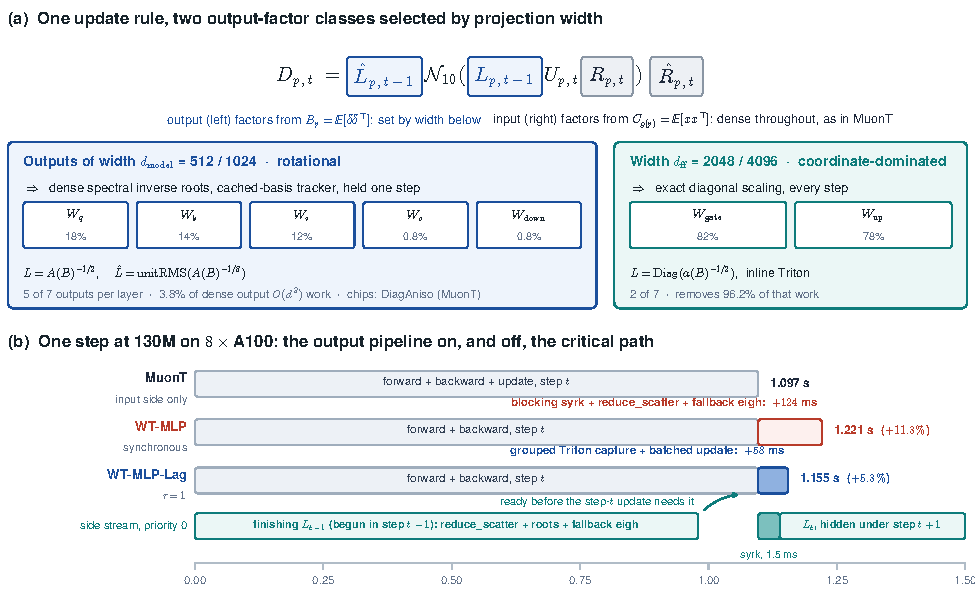
\includegraphics[width=\textwidth]{fig3_method_pipeline.pdf}
  \caption{\textbf{Factor assignment and execution pipeline of \mname{WT-MLP-Lag}.}
  \textbf{(a)} The four factor slots of \Cref{eq:update}. Right input factors stay dense for every projection, as in \mname{MuonT} (grey); the left output factor is chosen by the width of the cotangent, dense spectral roots at $\dm$ (blue) and exact per-step diagonal scaling at $\dff$ (teal). Chip labels give each moment's $\mathrm{DiagAniso}$ on the \mname{MuonT} trajectory (\Cref{tab:diagnosis}), the measurement that sets the threshold.
  \textbf{(b)} One training step at \texttt{130M} on $8\times\text{A100}$, drawn to scale from the median step times of \Cref{tab:bench19}. Synchronous two-sided execution appends \texttt{syrk}, \texttt{reduce\_scatter}, and fallback \texttt{eigh} to the step boundary, since $\delta_t$ exists only after backward completes. At $\tau=1$ the step-$t$ update instead consumes $L_{t-1}$, and the output pipeline runs on a priority-0 side stream: \texttt{syrk} ($\sim 1.5\text{ ms}$, guarded by \texttt{ev\_rows\_consumed}) followed by reduction and root updates for $L_t$ hidden under step $t+1$. Only the step bars are to scale; side-stream extents are schematic.}
  \label{fig:method_pipeline}
\end{figure}

\subsection{Systems Co-Design: Hiding Critical-Path Cotangent Latency}
\label{sec:systems}

Even after width thresholding removes $\dff$-wide eigendecompositions, executing five $\dm$-wide dense output roots synchronously (\mname{WT-MLP}) still adds $+11.3\%$ benchmark step-time overhead ($+21.9\%$ in early unbatched runs) because cotangents $\delta_t$ exist only \emph{after} backward completes (\Cref{fig:method_pipeline}b, middle row).
Our production engine (\texttt{fast\_lag}) eliminates this bottleneck via three orthogonal systems optimizations:

\paragraph{1. One-step asynchronous lag ($\tau = 1$), non-blocking masked repairs, and batched fallback \texttt{eigh}.}
In \mname{WT-MLP-Lag}, step $t$ applies step $t-1$'s already-computed output roots $(L_{p,t-1}, \hat{L}_{p,t-1})$ while keeping input roots $(R_{p,t}, \hat{R}_{p,t})$ current ($t=0$ uses identity left factors for $1$ step out of $5{,}120$).
At $\beta = 0.938$, a 1-step delay shifts the exponential weighting window by a single update out of $\approx 16.1$, costing $< 10^{-3}$ nats in held-out loss (\Cref{sec:ablations}).
Systems-wise, however, $\tau = 1$ moves the entire output pipeline off the critical path (\Cref{fig:method_pipeline}b, bottom two rows):
once backward $t$ finishes, a normal-priority ($\text{priority}=0$) CUDA side stream---chosen so background output work never preempts high-priority input roots or critical-path GEMMs---executes packed \texttt{syrk} ($\sim 1.5\text{ ms}$) and immediately records \texttt{ev\_rows\_consumed}, allowing step $t+1$'s backward pass to safely overwrite row buffers while \texttt{reduce\_scatter}, cached-basis iterations, and GPU fallback \texttt{eigh} overlap across the full forward/backward pass of step $t+1$.
Crucially, because cotangent subspaces trigger frequent fallbacks (\Cref{fig:structural_audit}c), naive per-round host flag synchronization (\texttt{.tolist()}) and per-matrix fallback loops would stall Python microbatch dispatch during step $t+1$; we eliminate both via 2-bit divergence gating (immediately skipping hopeless $\rho > \rho_{\max}$ repair rounds), non-blocking event-queried GPU-masked repairs (with power-of-two batch shapes pre-warmed at startup to prevent mid-run DDP recompilation stalls), single-call batched exact \texttt{eigh} fallbacks, and NUMA-isolated host basis-refresh worker pools.
To preserve exact temporal alignment across widths, diagonal \texttt{gate/up} roots are also held by one step, cached CUDA-graph root outputs are cloned before replay, and distributed checkpoints flush in-flight launches before serialization so continuous and resumed runs match to machine precision.

\paragraph{2. Grouped Triton backward capture, inline diagonals, and chunked row-buffer accumulation.}
In standard PyTorch autograd, attaching 224 per-projection \texttt{index\_select}/\texttt{index\_copy\_} hooks costs $92.9\text{ ms/step}$ and $1.8\text{ GiB}$ of BF16 row buffers at \texttt{130M} (and $>7\text{ GiB}$ unchunked at \texttt{520M}).
We replace these with (i) fused 2- and 3-way Triton store kernels at shared backward nodes (\texttt{q,k,v} and \texttt{gate,up}) for dense-tracked outputs, multiplying sampled BF16 rows by $2^{16}$ (exact exponent shift preventing FP32 squaring underflow before trace normalization), (ii) an \texttt{InlineDiagonalAccumulator} Triton split-reduction kernel that accumulates squared sampled cotangents for diagonal outputs directly into compact FP32 partial vectors during backward without materializing $\dff$-wide row buffers, and (iii) chunked row-buffer reuse (\texttt{root.chunk}), which flushes partial input and output Grams on side streams every $c$ microbatches ($c=2$ at \texttt{520M}), shrinking row-buffer memory by $87.5\%$ on $8\times\text{A100}$ and unlocking $2\times$ larger per-GPU microbatches within $40\text{ GB}$ HBM.
At \texttt{130M}, grouped capture cuts backward hook time by $8.4\times$ ($92.9 \to 11.1\text{ ms}$) and saves $1.1\text{ GiB}$ of peak memory.

\paragraph{3. Shape-batched updates with deduplicated Ozaki FP16-split Tensor-Core products.}
Following contiguous layer sharding ($4$ layers per rank on $8$ GPUs; $1$ layer per rank on $32$ GPUs), each rank stacks its owned matrices into three homogeneous 3D batches ($4\ell\times \dm \times \dm$, $2\ell\times \dff \times \dm$, $\ell\times \dm \times \dff$), deduplicates shared right-factor FP16 splits across grouped projections (\texttt{q,k,v} and \texttt{gate,up}), and executes batched $\Nten$ and root products via Ozaki-style high/low FP16-split Tensor-Core GEMMs~\citep{mohamadi2026toner}, achieving FP32 accuracy under deterministic \texttt{allow\_tf32=False} while cutting update-step overhead from $15.0\text{ ms}$ to $1.7\text{ ms}$, before \texttt{all\_gather}ing parameter deltas with zero-allocation in-place finite guards.

\section{Evaluation isolates the incremental output benefit}
\label{sec:protocol}

The comparison of interest is against tuned input-only MuonT. Its remaining loss gap is a few millinats, so learning-rate selection and numerical execution differences can be as large as the effect being measured. We use paired data ordering, an identity-factor execution control, and learning-rate sweeps at the full training budget before testing transfer.

\subsection{Models, budgets, and held-out losses}
\label{sec:testbed}

We train 32-layer, pre-RMSNorm SwiGLU Transformers on a 25.4B-token DCLM, StarCoderData, and Proof-Pile-2 mixture using the Marin PyTorch suite~\citep{mohamadi2026toner}. Runs use the Llama-3.1 vocabulary of 128,256 tokens, sequence length 4,096, document-isolated causal attention, and NVIDIA A100-40GB GPUs. Within each seed, optimizer arms share initialization and data ordering. The labels 130M and 520M refer to approximately 134M and 537M non-embedding parameters (\Cref{tab:regimes}).

\begin{table}[tbp]\centering\small
\setlength{\tabcolsep}{5.8pt}
\caption{\textbf{Pretraining regimes.} Params counts non-embedding parameters; TPP is tokens per non-embedding parameter. Fresh-seed confirmation uses seeds 1--3 after learning-rate selection and execution-path checks on seed 0.}\label{tab:regimes}
\begin{tabularx}{\textwidth}{@{}>{\raggedright\arraybackslash}Xrrrrrc@{}}
\toprule
Regime & Params & $\dm$ / $\dff$ & Tokens (TPP) & Batch / Steps & GPUs & Seeds \\
\midrule
130M controls \& LR bracket & 134M & 512 / 2,048 & 2.68B (20) & 0.5M / 5,120 & 8$\times$A100 & 0 \\
130M confirmation & 134M & 512 / 2,048 & 2.68B (20) & 0.5M / 5,120 & 8$\times$A100 & 1, 2, 3 \\
130M longer training & 134M & 512 / 2,048 & 10.74B (80) & 0.5M / 20,480 & 8$\times$A100 & 0 \\
520M width transfer & 537M & 1,024 / 4,096 & 10.74B (20) & 1.0M / 10,240 & 32$\times$A100 & 0 \\
\bottomrule\end{tabularx}
\end{table}


We report held-out training-mixture cross-entropy $\Lsel$, C4 loss $\Lc$, and the unweighted macro average over 16 Paloma domains $\Lpal$. Final losses measure completed models; paired means over 11 second-half checkpoints assess whether a difference persists through late training. Checkpoints from one trajectory are correlated observations and do not substitute for independent seeds. Figures report differences in millinats, where one millinat is $10^{-3}$ nats and negative differences favor the proposed method.

\subsection{Execution-path and learning-rate controls}
\label{sec:falsification}

Null-WT performs synchronous output capture, pooling, and root construction, then applies identity output factors. It controls the added numerical and collection path; it does not separately isolate asynchronous scheduling. It tests whether changes in tensor batching and mixed-precision accumulation can account for the measured gain. At learning rate 0.02263, its final loss is 0.0003 nats below MuonT, compared with a 0.0043-nat improvement for WT-MLP-Lag (\Cref{tab:controls}). The control makes execution-path drift an unlikely explanation for the full effect, although it is one measured control rather than a proof of numerical equivalence.

\begin{figure}[t]
 \centering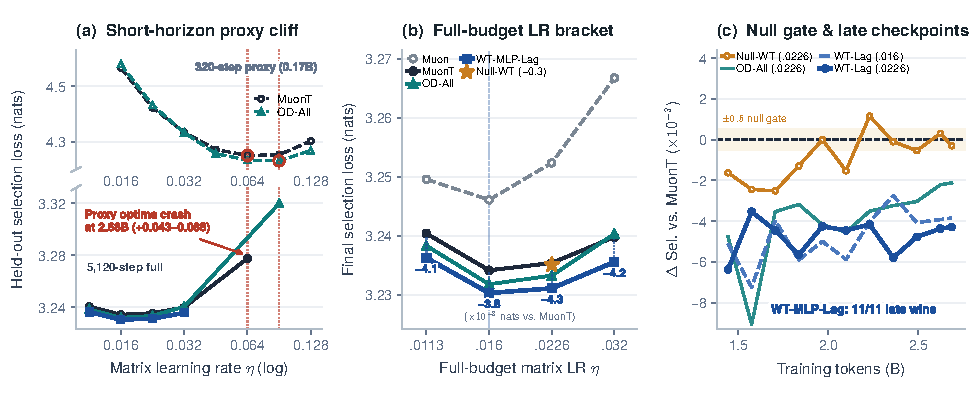
\includegraphics[width=\textwidth]{fig4_confounds_lr_null.pdf}
 \caption{\textbf{The gain survives full-budget tuning and an execution-path control.}
 \textbf{(a)} Learning rates selected on a 320-step schedule transfer poorly to the full budget.
 \textbf{(b)} Full-budget held-out loss across a learning-rate bracket, with a matched-path identity-factor control (Null-WT).
 \textbf{(c)} Late-training differences from MuonT at learning rate 0.02263: the control stays much closer to MuonT than WT-MLP-Lag does. All panels use 130M, seed 0; the full budget is 2.68B tokens.}
 \label{fig:confounds}
\end{figure}

\begin{table}[tbp]\centering\small
\setlength{\tabcolsep}{5.2pt}
\caption{\textbf{Seed-0 learning-rate bracket, execution-path control, and short-schedule transfer at 130M (2.68B tokens).} Entries are final held-out losses in nats across the complete four-point bracket (bold marks each row's full-budget minimum, $\eta^*=0.0160$ for every method); $\Delta_{0.0226}$ is the paired difference from MuonT at $\eta=0.02263$ in millinats where Null-WT is evaluated. The rightmost column transfers each checked arm's 320-step argmax learning rate (\Cref{tab:lr_cliff}) to the full 5,120-step schedule.}\label{tab:controls}
\begin{tabularx}{\textwidth}{@{}>{\raggedright\arraybackslash}Xrrrrrr@{}}
\toprule
& \multicolumn{4}{c}{Full-budget held-out loss $\Lsel$ (nats)} & & \\
\cmidrule(lr){2-5}
Method & $0.0113$ & $0.0160$ & $0.0226$ & $0.0320$ & $\Delta_{0.0226}$ (mnats) & 320-step $\eta^* \to$ full \\
\midrule
Muon & 3.2496 & \textbf{3.2461} & 3.2524 & 3.2667 & $+16.96$ & --- \\
MuonT & 3.2404 & \textbf{3.2342} & 3.2354 & 3.2398 & $+0.00$ & $0.0640 \to 3.2775$ \\
Null-WT (ctrl) & --- & --- & 3.2351 & --- & $-0.30$ & --- \\
OD-All & 3.2383 & \textbf{3.2318} & 3.2333 & 3.2403 & $-2.13$ & $0.0905 \to 3.3200$ \\
\rowcolor{rowtint}[0pt][0pt]\textbf{WT-MLP-Lag} & 3.2363 & \textbf{3.2303} & 3.2311 & 3.2356 & $\mathbf{-4.29}$ & --- \\
\bottomrule\end{tabularx}
\end{table}


Learning rates selected on a short schedule do not transfer reliably to the full budget. A 320-step sweep favors rates of 0.064--0.0905, three to four times the useful full-budget scale. Transferring those choices to 5,120 steps worsens final loss by 0.04--0.09 nats in the checked arms, overwhelming the output-side gain. This is consistent with broader concerns about optimizer comparisons across tuning budgets and horizons~\citep{choi2019empirical,schmidt2021crowded,kaddour2023nodata,dang2026batchsize}.

We therefore sweep $\eta\in\{0.01131,0.016,0.02263,0.032\}$ across all four core methods at the full 2.68B-token budget (\Cref{fig:confounds}(b),\Cref{tab:controls}). Every method achieves a strict interior minimum at $\eta^*=0.016$, rising on both the cooler ($\eta=0.01131$) and hotter ($\eta\ge0.02263$) sides, while WT-MLP-Lag improves on MuonT at every matched rate by 0.0038--0.0043 nats. Sharing the same full-budget optimum allows fresh-seed confirmation across all four methods at a common learning rate without schedule confounds; we also record the hotter $\eta=0.02263$ replicates for OD-All and WT-MLP-Lag in \Cref{app:appendix_lr}.

\section{The gain persists with more data and greater width}
\label{sec:scaling}

WT-MLP-Lag lowers final loss relative to MuonT in all three training regimes. The improvement is small in absolute units, but adds 29--43\% to the held-out gain that input preconditioning already obtains over Muon. For held-out loss, the relative extension is $(\mathcal L_{\rm MuonT}-\mathcal L_{\rm WT})/(\mathcal L_{\rm Muon}-\mathcal L_{\rm MuonT})$. Its denominator is 0.0119, 0.0103, and 0.0065 nats in the three regimes. The direct differences in \Cref{tab:main_scaling} show the effect size and replication level.

\begin{table}[!htb]\centering\small
\setlength{\tabcolsep}{2.2pt}
\caption{\textbf{Confirmatory and scaling results across fresh seeds, longer horizon, and greater width.} Held-out reports final cross-entropy $\Lsel$ in nats; all $\Delta$ columns report differences from same-regime Muon in millinats (negative favors the row method). MuonT applies input preconditioning only, so the gap between the MuonT and WT-MLP-Lag rows isolates the output-side contribution. Late-11 averages the 11 second-half checkpoints; Wins counts the 16 Paloma domains improved over Muon. At 130M, all four methods share their bracketed seed-0 optimum ($\eta^*=0.01600$ at 20 TPP and $0.01600\times4^{-0.3}=0.01056$ at 80 TPP); at 520M Muon runs at its own selected rate while the preconditioned methods share MuonT's pinned rate, so that block compares each method at its chosen rate rather than at a matched one. Complete absolute losses and $\eta=0.02263$ replicates appear in \Cref{tab:absolute_results,tab:seeds}.}\label{tab:main_scaling}
\begin{tabularx}{\textwidth}{@{}>{\raggedright\arraybackslash}Xrrrrrrr@{}}
\toprule
& & (nats) & \multicolumn{4}{c}{Differences from Muon (millinats, $\downarrow$)} & Paloma \\
\cmidrule(lr){4-7}
Method & LR $\eta$ & Held-out & $\Delta$ Held-out & Late-11 $\Delta$ & $\Delta$ C4 & $\Delta$ Paloma & Wins \\
\midrule
\addlinespace[2pt]\multicolumn{8}{@{}l}{\textit{130M confirmation: 20 TPP, 2.68B tokens, fresh seeds 1--3 (matched $\eta^*=0.0160$, paired mean $\pm$ SD)}}\\
Muon & 0.01600 & 3.2035 & $+0.00$ & $+0.00$ & $+0.00$ & $+0.00$ & --- \\
MuonT & 0.01600 & 3.1916 & $-11.91\pm1.40$ & $-23.26\pm2.07$ & $-11.79\pm0.98$ & $-11.49\pm4.18$ & 16/16 \\
OD-All & 0.01600 & 3.1919 & $-11.62\pm1.09$ & $-22.91\pm1.63$ & $-12.63\pm1.22$ & $-12.79\pm1.92$ & 16/16 \\
\rowcolor{rowtint}[0pt][0pt]\textbf{WT-MLP-Lag} & 0.01600 & \textbf{3.1881} & $\mathbf{-15.41\pm2.18}$ & $\mathbf{-26.78\pm2.30}$ & $\mathbf{-15.64\pm1.80}$ & $\mathbf{-15.91\pm1.68}$ & \textbf{16/16} \\
\addlinespace[5pt]\multicolumn{8}{@{}l}{\textit{130M longer training: 80 TPP, 10.74B tokens, seed 0 (matched rate)}}\\
Muon & 0.01056 & 3.0778 & $+0.00$ & $+0.00$ & $+0.00$ & $+0.00$ & --- \\
MuonT & 0.01056 & 3.0675 & $-10.28$ & $-22.28$ & $-10.26$ & $-11.12$ & 15/16 \\
OD-All & 0.01056 & 3.0656 & $-12.19$ & $-23.85$ & $-12.82$ & $-13.71$ & 16/16 \\
\rowcolor{rowtint}[0pt][0pt]\textbf{WT-MLP-Lag} & 0.01056 & \textbf{3.0636} & $\mathbf{-14.23}$ & $\mathbf{-26.82}$ & $\mathbf{-14.07}$ & $\mathbf{-16.78}$ & \textbf{16/16} \\
\addlinespace[5pt]\multicolumn{8}{@{}l}{\textit{520M width transfer: 20 TPP, 10.74B tokens, $\dm=1{,}024$, seed 0 (pinned rate)}}\\
Muon & 0.01600 & 2.8528 & $+0.00$ & $+0.00$ & $+0.00$ & $+0.00$ & --- \\
MuonT & 0.02263 & 2.8463 & $-6.45$ & $-1.87$ & $-6.49$ & $-3.49$ & 15/16 \\
OD-All & 0.02263 & 2.8469 & $-5.88$ & $-1.28$ & $-6.09$ & $-3.02$ & 14/16 \\
\rowcolor{rowtint}[0pt][0pt]\textbf{WT-MLP-Lag} & 0.02263 & \textbf{2.8435} & $\mathbf{-9.25}$ & $\mathbf{-4.92}$ & $\mathbf{-8.71}$ & $\mathbf{-8.93}$ & \textbf{15/16} \\
\bottomrule\end{tabularx}
\end{table}


\subsection{Fresh seeds confirm an incremental benefit}
\label{sec:phase2}

On fresh 130M seeds 1--3 at the shared full-budget optimum $\eta^*=0.016$, WT-MLP-Lag improves on MuonT on every seed across held-out mixture, C4, and Paloma macro loss, as well as across late-training checkpoints (\Cref{tab:main_scaling}). Its paired held-out improvement is $0.0035\pm0.0017$ nats (mean $\pm$ sample standard deviation across seeds), whereas OD-All leaves held-out mixture loss essentially unchanged ($+0.0003\pm0.0004$ nats). Repeating both output methods on the same seeds at $\eta=0.02263$ yields the same ranking ($0.0034\pm0.0015$ versus $0.0005\pm0.0005$ nats; \Cref{tab:absolute_results,tab:seeds}). Retaining cross-channel correlations at hidden width therefore accounts for the 130M gain rather than learning-rate selection or coordinate scaling alone.

The improvement also survives a doubled global batch of 1M tokens: the checked run gains 0.0036 nats on held-out mixture and 0.0040 nats on C4 relative to MuonT. This is a batch-size check, not an additional multi-seed confirmation.

\subsection{Longer training retains the gain at matched learning rates}
\label{sec:phase3}

Training 130M for 10.74B tokens tests whether MuonT catches up once the token budget grows fourfold. At a shared learning rate of 0.01056, WT-MLP-Lag finishes 0.0040 nats lower on held-out mixture and stays ahead at every second-half checkpoint. Its Paloma macro gain is 0.0057 nats, with improvements on all 16 domains. The fixed-token advantage therefore persists through the 80-TPP schedule in this seed.

The shared rate $\eta=0.016\times4^{-0.3}=0.01056$ scales the common 20-TPP optimum to the fourfold horizon. Scaling from the hotter $\eta=0.02263$ grid point instead ($\eta=0.01493$, $\sqrt2\times$ higher) develops a mid-training penalty and finishes worse on Paloma (\Cref{fig:scaling_traj}(b),\Cref{tab:absolute_results}). A useful output approximation therefore does not remove sensitivity to horizon-scaled learning rates.

\begin{figure}[t]
 \centering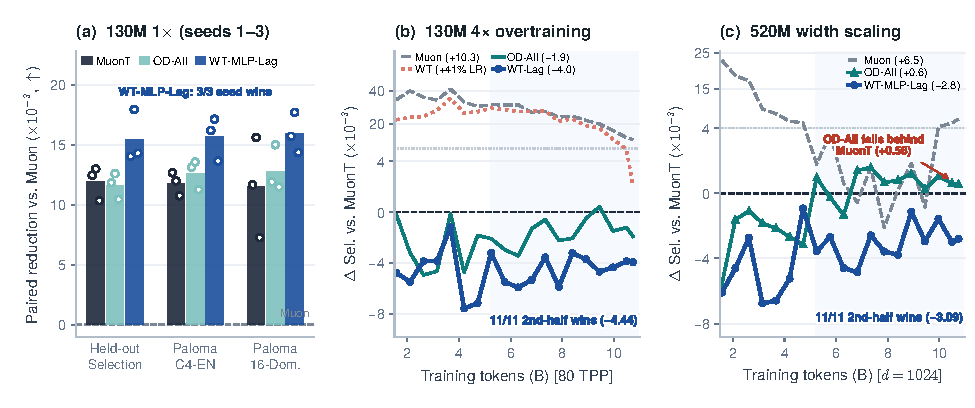
\includegraphics[width=\textwidth]{fig5_scaling_trajectories.pdf}
 \caption{\textbf{The width-thresholded gain survives fresh seeds, longer training, and greater width.}
 \textbf{(a)} Final loss reductions versus same-seed Muon at 130M, 20 TPP. Bars show three-seed means; open circles show individual seeds.
 \textbf{(b, c)} Held-out differences from MuonT during the 10.74B-token runs: 130M at 80 TPP and 520M at 20 TPP, each with one seed. The hotter WT run in (b) shows learning-rate sensitivity. Vertical axes compress the positive range above the dotted lines; negative differences indicate lower loss.}
 \label{fig:scaling_traj}
\end{figure}

\subsection{Wider models expose the limit of all-diagonal outputs}
\label{sec:phase4}

Doubling hidden width to 1,024 separates the two output approximations. OD-All finishes slightly worse than MuonT on held-out mixture, C4, and Paloma macro loss. WT-MLP-Lag instead improves held-out loss by 0.0028 nats and remains ahead at all 11 late checkpoints. All three preconditioned methods use MuonT's pinned 520M rate of 0.02263, with no output-side retuning.

The out-of-distribution evaluation supports the same distinction. WT-MLP-Lag improves on MuonT in 15 of 16 Paloma domains; OD-All improves in six. The domain plot exposes both the spread of gains and the remaining regression instead of relying only on a macro average (\Cref{fig:paloma}). Since domains share training and evaluation influences, these win counts describe coverage rather than independent replications.

\begin{figure}[t]
 \centering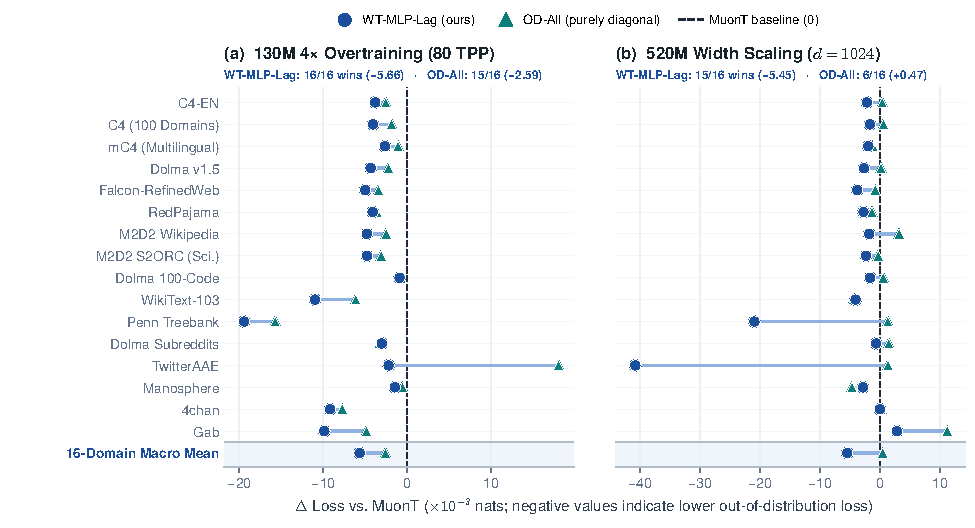
\includegraphics[width=\textwidth]{fig6_paloma_domains.pdf}
 \caption{\textbf{Most Paloma domains benefit from retaining dense hidden-width outputs.}
 Final per-domain loss differences from MuonT. \textbf{(a)} At 130M, 80 TPP, WT-MLP-Lag wins 16/16 domains. \textbf{(b)} At 520M, 20 TPP, it wins 15/16 and OD-All wins 6/16. Circles denote WT-MLP-Lag; triangles denote OD-All. The bottom row gives the unweighted macro mean. Panels use different horizontal scales; connecting lines compare methods within a domain and are not confidence intervals. Each regime uses one seed.}
 \label{fig:paloma}
\end{figure}

Two widths do not establish an asymptotic scaling law. We next test the proposed directional explanation on saved checkpoints.

\section{Design-Space Ablations, Related Preconditioners, and Mechanism}
\label{sec:analysis}

Having established \emph{that} \mname{WT-MLP-Lag} improves fixed-token pretraining across seeds, horizons, and widths, we now answer \emph{why} each component of its design is necessary:
we ablate factor placement across all 19 taxonomic variants (\Cref{sec:ablations}), compare head-to-head against recent curvature-aware polar optimizers \mname{GO-MUON} and \mname{Mousse} (\Cref{sec:related_baselines}), verify via counterfactual direction grafting that output roots act by subspace rotation rather than step-size inflation (\Cref{sec:mechanism}), and map the multi-scale \texttt{130M} and \texttt{520M} quality--wall-clock Pareto frontiers (\Cref{sec:pareto}).

\subsection{Controlled Factor-Placement and Approximation Ablations}
\label{sec:ablations}

\Cref{tab:ablations} and \Cref{fig:ablations_related}a isolate five structural design questions on matched \texttt{130M} ($2.68\text{B}$-token, \texttt{seed 0}) trajectories:

\begin{enumerate}[leftmargin=1.6em, itemsep=2pt, topsep=2pt]
  \item \textbf{Output preconditioning is complementary to, never a substitute for, input whitening.}
  Replacing input factors with dense output factors everywhere (\mname{Abl-OutOnly}, mirror image of \mname{MuonT}) degrades late $\Lsel$ by $+0.0087$ nats---performing even worse than unpreconditioned \mname{Muon} ($+0.0055$)!
  Even swapping only $W_{\mathrm{down}}$'s $2{,}048$-wide input root for a $512$-wide output root (\mname{Abl-DownSwap}) loses $+0.0025$ nats.
  Similarly, diagonalizing \emph{both} sides (\mname{Abl-BothDiag}) loses $+0.0180$ nats because $\dm$-wide inputs carry $>98\%$ rotational anisotropy (\Cref{tab:diagnosis}).
  \item \textbf{Diagonalizing \texttt{gate,up} matches or slightly exceeds full dense outputs, whereas dropping them halves the gain.}
  Comparing \mname{WT-MLP} ($-0.0066$ late $\Lsel$) against full dense \mname{DT-All} ($-0.0058$) confirms that removing $\dff$-wide output rotations sacrifices \emph{zero} held-out quality---in fact edging slightly ahead because exact per-step diagonal scaling avoids 4-step cached-basis staleness on rapidly drifting \texttt{gate/up} moments while cutting rank-0 exact fallbacks by $39\%$ ($32{,}838 \to 19{,}998$).
  Conversely, omitting \texttt{gate/up} output factors altogether (\mname{Abl-No2048}) forfeits over half the gain ($-0.0031$ vs.\ $-0.0066$), proving that pre-SwiGLU coordinate scale carries genuine optimization signal.
  \item \textbf{Both inner ($-1/2$) and outer ($-1/8$) left factors contribute.}
  Applying dense left factors only \emph{outside} $\Nten$ (\mname{Abl-OuterDense}, $L=I$) drops late $\Lsel$ gain from $-0.0058$ to $-0.0040$ (and diagonal outer-only \mname{OD-Outer} drops from $-0.0029$ to $-0.0020$ in fixed-age Wave 7), demonstrating that pre-$\Nten$ singular-frame rotation accounts for roughly one-third of the benefit.
  \item \textbf{Asymmetric (\mname{WT-MLP-Lag}) vs.\ symmetric (\mname{WT-Sym-Lag}) $\dff$ thresholding.}
  What if we apply the exact same width rule symmetrically to the input side by also diagonalizing $\dff$-wide \texttt{in:down} (\mname{WT-Sym-Lag})?
  In a same-wave head-to-head run (\texttt{wave\_sym\_fastlag}), \mname{WT-Sym-Lag} cuts benchmark step overhead to just $+3.32\%$ ($20.82\text{ GiB}$ peak memory) and still beats \mname{MuonT} at completion ($-0.0025$ final $\Lsel$, $-0.0029$ final $\Lc$), \emph{but} lags \mname{WT-MLP-Lag} by $+0.0181 \pm 0.0024$ nats in the first $537\text{M}$-token training window and $+0.0036$ nats in late $\Lsel$.
  Why? Unlike pre-SwiGLU \texttt{out:gate,up} ($\rho_{\mathrm{rms}} = 0.0048\text{--}0.0082$, $77.9\%\text{--}90.8\%$ diagonal anisotropy), post-SwiGLU \texttt{in:down} retains $56.6\%\text{--}79.7\%$ off-diagonal moment anisotropy across \mname{Muon}, \mname{MuonT}, and \mname{WT-MLP-Lag} ($\rho_{\mathrm{rms}} = 0.0283 / 0.0346 / 0.0359$; \Cref{tab:diagnosis}) that substantially accelerates early-stage descent.
  \item \textbf{One-step asynchronous lag ($\tau = 1$) is nearly lossless.}
  Update-by-update paired differencing over the final $537\text{M}$ tokens shows \mname{WT-MLP-Lag} differs from synchronous \mname{WT-MLP} by just $+0.00011 \pm 0.00004$ nats in training loss ($+0.00033$ final $\Lsel$ in Wave 4; and \mname{DT-All-Lag} matches \mname{DT-All} to $-0.0001$ late $\Lsel$) while halving step-time overhead.
\end{enumerate}

\begin{table}[t]
  \centering
  \caption{\textbf{Controlled factor-placement and approximation ablations at \texttt{130M}} ($0.5\text{M}$ batch, $5{,}120$ steps, $2.68\text{B}$ tokens, \texttt{seed 0}, $\eta = 0.02263$ [$\eta=0.016$ for \mname{Muon}]). ``Late $\Delta\Lsel$'' and ``Late $\Delta\Lc$'' average the 11 second-half evaluations ($\text{steps } 2{,}751\text{--}5{,}120$) relative to \mname{MuonT}; ``$\Delta\mathcal{L}_{\mathrm{train}}$'' is the exact per-update paired training loss difference over the final $537\text{M}$ tokens ($\text{SE} \approx 0.00004\text{--}0.00016$); ``Bench $\Delta t$'' is the unified 8-GPU step-time overhead vs.\ \mname{MuonT} (\texttt{bench\_8gpu\_opt}).}
  \label{tab:ablations}
  \vspace{2pt}
  \resizebox{\textwidth}{!}{%
  \begin{tabular}{@{}llllrrrr@{}}
    \toprule
    Method & Right ($R,\hat{R}$) & Left ($L,\hat{L}$: $\dm \,/\, \dff$) & Special Setting & Late $\Delta\Lsel$ & Late $\Delta\Lc$ & $\Delta\mathcal{L}_{\mathrm{train}}$ & Bench $\Delta t$ \\
    \midrule
    \mname{Abl-BothDiag}   & Diag / Diag   & Diag / Diag   & Both sides diagonal & $+0.0180$ & $+0.0177$ & $+0.0134$ & $-0.4\%$ \\
    \mname{Abl-OutOnly}    & $I$ / $I$     & Dense / Dense & Drop all inputs     & $+0.0087$ & $+0.0109$ & $+0.0079$ & $+29.8\%$ \\
    \mname{Muon}           & $I$ / $I$     & $I$ / $I$     & $\eta = 0.016$      & $+0.0055$ & $+0.0053$ & $+0.0062$ & $-1.4\%$ \\
    \mname{Abl-DownSwap}   & $\text{down}\!=\!I$ & $\text{down}$ Dense & Swap \texttt{down} in$\to$out & $+0.0025$ & $+0.0036$ & $+0.0032$ & $+0.3\%$ \\
    \midrule
    \mname{MuonT}          & Dense / Dense & $I$ / $I$     & Reference baseline  & $0.0000$  & $0.0000$  & $0.0000$  & $0.0\%$ \\
    \mname{Null-WT}        & Dense / Dense & $(I, I)$ applied & Same-wave null   & $-0.0007$ & $-0.0009$ & $-0.0005$ & $+12.3\%$ \\
    \midrule
    \mname{Abl-DownOnly}   & Dense / Dense & $\hat{L}_{\mathrm{down}}$ only & \texttt{down} outer only & $-0.0014$ & $-0.0008$ & $-0.0012$ & $+2.1\%$ \\
    \mname{WT-Sym-Lag}     & Dense / Diag  & Dense / Diag  & $\tau=1$, sym.\ $\dff$ & $-0.0011$ & $-0.0016$ & $-0.0015$ & $+3.3\%$ \\
    \mname{WT-Sym}         & Dense / Diag  & Dense / Diag  & $\tau=0$, sym.\ $\dff$ & $-0.0025$ & $-0.0020$ & $-0.0013$ & $+9.3\%$ \\
    \mname{Abl-No2048}     & Dense / Dense & Dense / $I$   & Drop \texttt{gate,up} & $-0.0031$ & $-0.0026$ & $-0.0021$ & $+12.0\%$ \\
    \mname{Abl-OuterDense} & Dense / Dense & $\hat{L}$ Dense ($L\!=\!I$) & Outer $-1/8$ only & $-0.0040$ & $-0.0048$ & $-0.0039$ & $+26.4\%$ \\
    \mname{OD-All}         & Dense / Dense & Diag / Diag   & All outputs diag    & $-0.0045$ & $-0.0036$ & $-0.0037$ & $+2.2\%$ \\
    \rowcolor{rowtint}
    \textcolor{colWT}{\mname{WT-MLP-Lag}} & Dense / Dense & Dense / Diag & $\tau=1$ lag (ours) & \textbf{$-$0.0057} & \textbf{$-$0.0050} & \textbf{$-$0.0050} & \textbf{+5.3\%} \\
    \mname{DT-All}         & Dense / Dense & Dense / Dense & $\tau=0$ dense ceil. & $-0.0058$ & $-0.0064$ & $-0.0050$ & $+21.6\%$ \\
    \mname{DT-All-Lag}     & Dense / Dense & Dense / Dense & $\tau=1$ dense ceil. & $-0.0059$ & $-0.0059$ & $-0.0057$ & $+16.6\%$ \\
    \rowcolor{rowtint}
    \textcolor{colWT}{\mname{WT-MLP}}     & Dense / Dense & Dense / Diag & $\tau=0$ sync (ours) & \textbf{$-$0.0066} & \textbf{$-$0.0061} & \textbf{$-$0.0051} & $+11.3\%$ \\
    \bottomrule
  \end{tabular}%
  }
\end{table}

\begin{figure}[t]
  \centering
  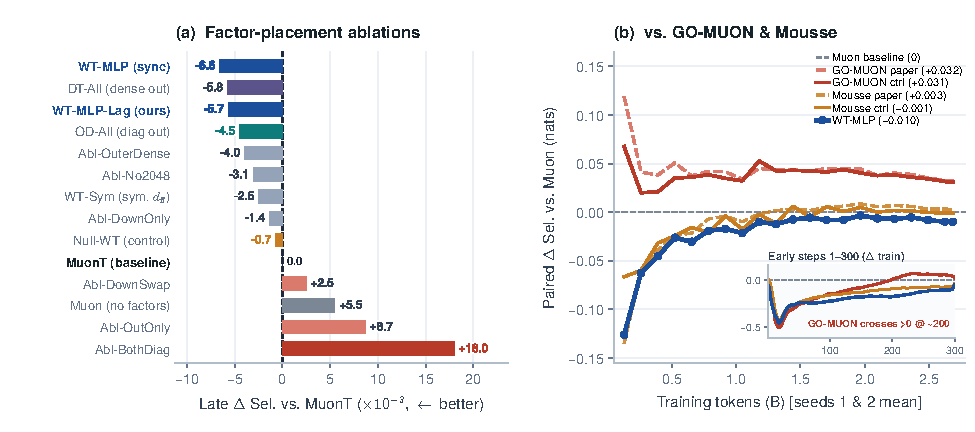
\includegraphics[width=\textwidth]{fig7_ablations_and_related.pdf}
  \caption{\textbf{Design-space ablations and multi-seed comparison against recent polar preconditioners.}
  Unlike \Cref{tab:main_scaling}, differences here are reported against same-wave \mname{MuonT}: these arms vary only the output-side operator at a fixed dense input side, so \mname{MuonT} is the controlled reference. For reference, \mname{MuonT} itself is $-0.0119$ nats below \mname{Muon} in this regime.
  \textbf{(a)} Late-half $\Delta\Lsel$ vs.\ \mname{MuonT} across 14 controlled configurations at \texttt{130M} ($2.68\text{B}$ tokens), showing that dropping input whitening (\mname{Abl-OutOnly}, \mname{Abl-BothDiag}) degrades loss, whereas width-thresholded \mname{WT-MLP} and \mname{WT-MLP-Lag} match or exceed full dense \mname{DT-All}.
  \textbf{(b)} Paired held-out $\Delta\Lsel$ vs.\ \mname{Muon} (mean across fresh \texttt{seeds 1 \& 2}, isotropic matrix decay, $\eta = 0.032$). Inset shows 9-step smoothed early training loss deltas ($\text{steps } 1\text{--}300$): \mname{GO-MUON} plunges $-0.57$ nats by step $18$ before crossing above \mname{Muon} around step $200$ and finishing $+0.031\text{--}0.032$ nats worse, while \mname{Mousse} tracks \mname{Muon} ($\pm 0.003$) and \mname{WT-MLP} maintains a steady $-0.010$-nat lead.}
  \label{fig:ablations_related}
\end{figure}

\subsection{Comparison with Curvature-Aware Polar Baselines (\mname{GO-MUON} and \mname{Mousse})}
\label{sec:related_baselines}

We next benchmark width-thresholded preconditioning against the two closest two-sided polar preconditioners in recent literature:
\mname{GO-MUON}~\citep{che2026gomuon}, which forms activation and observed-cotangent moments with Oracle Approximating Shrinkage (OAS), applies symmetric inverse \emph{quarter} powers $P_B = B^{-1/4}, P_A = C^{-1/4}$ both inside and outside polar orthogonalization, and grafts the result to Frobenius norm $\sqrt{\min(m,n)}$; and
\mname{Mousse}~\citep{zhang2026mousse}, which avoids activation/cotangent hooks by maintaining Shampoo-style weight-gradient Gram EMAs ($G G^{\Tr}, G^{\Tr} G$) with symmetric $-1/8$ powers in eigen-coordinates and post-NS norm grafting.

To separate mathematical geometry from implementation details, we evaluate \emph{both} a controlled profile (sharing our runner's EMA $\beta=0.938$, ridge, refresh cadence, and $\Nten$) and a paper-adapter profile (\mname{GO-MUON}'s OAS shrinkage, compact-SVD polar, and $\beta_B=0.97$ sparse backward EMA; \mname{Mousse}'s pinned 5-stage BF16 polynomial and $\sqrt{m/n}$ scaling), alongside same-runner \mname{Muon} and \mname{WT-MLP} under uniform isotropic matrix weight decay ($\lambda = 0.1$).
After screening all 6 arms across 3 learning rates ($18$ seed-0 runs; every arm selected $\eta = 0.032$), we ran $12$ full-budget ($5{,}120$-step, $2.68\text{B}$-token) confirmations across fresh \texttt{seeds 1 and 2} (\Cref{tab:related}, \Cref{fig:ablations_related}b).

\begin{table}[t]
  \centering
  \caption{\textbf{Controlled multi-seed comparison against \mname{GO-MUON} and \mname{Mousse}} at \texttt{130M} ($2.68\text{B}$ tokens, $5{,}120$ steps, isotropic matrix weight decay $\lambda=0.1$, short-screened $\eta=0.032$, mean across fresh \texttt{seeds 1 \& 2}; standalone synchronous reference harness where ``Total $\Delta t$'' reflects full $5{,}120$-step end-to-end wall-clock time including evaluations).}
  \label{tab:related}
  \vspace{2pt}
  \resizebox{\textwidth}{!}{%
  \begin{tabular}{@{}llrrrrrr@{}}
    \toprule
    Method & Moment Source \& Power Split & Final $\Lsel$ & $\Delta\Lsel$ vs.\ \mname{Muon} & Late $\Delta\Lsel$ & Final $\Lc$ & Step (s) & Total $\Delta t$ \\
    \midrule
    \mname{Muon} (control)  & None; $\Nten(U_t)$                       & $3.2074$ & $0.0000$  & $0.0000$  & $3.4841$ & $1.153$ & $0.0\%$ \\
    \mname{Mousse} (paper)  & Grad Grams $G G^{\Tr}, G^{\Tr}G$; $(-1/8,-1/8)$ & $3.2102$ & $+0.0028$ & $+0.0049$ & $3.4873$ & $1.125$ & $+9.8\%$ \\
    \mname{Mousse} (ctrl)   & Grad Grams $G G^{\Tr}, G^{\Tr}G$; $(-1/8,-1/8)$ & $3.2064$ & $-0.0010$ & $+0.0012$ & $3.4822$ & $1.202$ & $+32.7\%$ \\
    \mname{GO-MUON} (ctrl)  & $C_t, B_t$; $(-1/4,-1/4)$ + norm graft   & $3.2384$ & $+0.0310$ & $+0.0382$ & $3.5135$ & $1.588$ & $+52.0\%$ \\
    \mname{GO-MUON} (paper) & OAS $C_t, B_t$; SVD polar + norm graft   & $3.2395$ & $+0.0321$ & $+0.0397$ & $3.5146$ & $2.021$ & $+94.3\%$ \\
    \rowcolor{rowtint}
    \textcolor{colWT}{\mname{WT-MLP}} & $C_t, B_t$ ($\dff$ diag); $(-1/2,-1/8)$ unit-RMS & \textbf{3.1975} & \textbf{$-$0.0099} & \textbf{$-$0.0071} & \textbf{3.4742} & $1.365$ & $+21.1\%$ \\
    \bottomrule
  \end{tabular}%
  }
\end{table}

Two sharp lessons stand out in \Cref{tab:related} and \Cref{fig:ablations_related}b:
\begin{itemize}[leftmargin=1.5em, itemsep=2pt, topsep=2pt]
  \item \textbf{Why \mname{GO-MUON} dives early then inverts:} During the first $20$ updates, both \mname{GO-MUON} profiles plunge $-0.50$ to $-0.64$ nats below \mname{Muon} (\Cref{fig:ablations_related}b inset), explaining their strong appeal on short-horizon tasks. However, both cross \emph{above} \mname{Muon} around step $180\text{--}210$ and finish $+0.0310$ and $+0.0321$ nats worse at $2.68\text{B}$ tokens ($+52\%\text{--}94\%$ slower). Applying a steep $-1/4$ power \emph{outside} polar orthogonalization coupled with forced $\sqrt{\min(m,n)}$ Frobenius norm grafting over-amplifies noisy cotangent directions once initial transient curvature subsides---validating \mname{MuonT} and \mname{WT-MLP}'s decoupled $(-1/2 \text{ inner},\,-1/8 \text{ outer})$ exponent split.
  \item \textbf{Decoupled moments beat entangled gradient Grams:} \mname{Mousse} finishes within $-0.0010$ (controlled) and $+0.0028$ (paper) of \mname{Muon}, whereas \mname{WT-MLP} outperforms \mname{Muon} by $-0.0099$ nats ($-0.0089$ over \mname{Mousse-Ctrl} on both seeds; also showing that \mname{WT-MLP} retains strong gains under isotropic weight decay). Because $G = \sum_j \delta_j x_j^{\Tr}$, gradient Grams $G G^{\Tr}$ entangle output cotangents with squared activation norms $\|x_j\|_2^2$ and cross-sample interference, losing the clean Kronecker separation of $C_t$ and $B_t$.
\end{itemize}

\subsection{Mechanistic Verification: Subspace Rotation vs.\ Step-Size Scaling}
\label{sec:mechanism}

Recent critiques of spectral optimizers (\citealt{shumaylov2026freon}; \citealt{goyal2026spectrally}) show that apparent geometric gains can stem covertly from altering the effective step-size norm $\|D_t\|_F / \|W_t\|_F$.
To test this hypothesis directly, we perform a counterfactual direction-grafting audit on saved mid-training (step $2{,}500$) and final (step $5{,}120$) checkpoints: holding \mname{MuonT}'s exact weights $W_t$, Nesterov source $U_t$, and right factors $(R_t, \hat{R}_t)$ fixed, we compute the counterfactual update $D_{\text{cand}}$ under \mname{WT-MLP}, \mname{OD-All}, and \mname{DT-All} and compare its Frobenius norm and angle $\theta(D_{\text{cand}}, D_{\text{MuonT}}) = \arccos\frac{\langle D_{\text{cand}}, D_{\text{MuonT}}\rangle}{\|D_{\text{cand}}\|_F \|D_{\text{MuonT}}\|_F}$ across all $224$ matrices (\Cref{fig:mech_pareto}a):

\begin{itemize}[leftmargin=1.5em, itemsep=2pt, topsep=2pt]
  \item \textbf{Zero step-size inflation:} \mname{WT-MLP}'s unit-RMS outer factors slightly \emph{reduce} update Frobenius norm relative to \mname{MuonT} ($\|D_{\text{WT}}\|_F / \|D_{\text{MuonT}}\|_F = 0.9854$, or $-1.46\%$ at step $2{,}500$ and $-1.91\%$ at step $5{,}120$; realized block weight norms are $-2.45\%$ to $-3.00\%$ smaller, vs.\ $-0.11\%$ for \mname{Null-WT}), while rotating update directions by a mean angle of $22.4^\circ$ ($\cos = 0.9218$, nearly matching full dense \mname{DT-All}'s $22.8^\circ$).
  \item \textbf{Mechanistic explanation for \mname{OD-All} falling back onto \mname{MuonT} at \texttt{520M}:} Inspecting rotation angles projection-by-projection (\Cref{fig:mech_pareto}a) reveals that on \texttt{gate} and \texttt{up}, \mname{OD-All} and \mname{WT-MLP} induce nearly identical rotations ($\sim 23^\circ\text{--}26^\circ$; counterfactual $\cos(D_{\text{diag}}, D_{\text{dense}}) = 0.988$ and $0.972$ median). On residual-stream writers \texttt{o} and \texttt{down}, however, \mname{OD-All} rotates \mname{MuonT}'s update by only $4.3^\circ$ and $5.4^\circ$, whereas \mname{WT-MLP} rotates them by $17.7^\circ$ and $17.0^\circ$! Thus \mname{OD-All} leaves residual-stream updates nearly unpreconditioned on the left---a deficit that becomes decisive at width $d = 1{,}024$.
\end{itemize}

\begin{figure}[t]
  \centering
  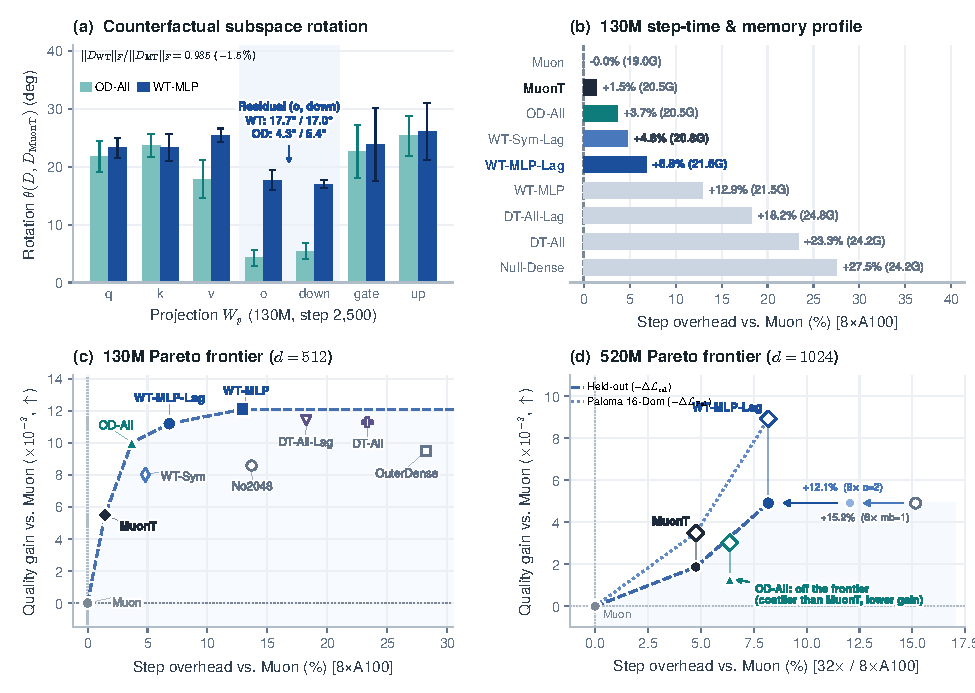
\includegraphics[width=\textwidth]{fig8_mechanism_and_pareto.pdf}
  \caption{\textbf{Mechanistic verification and multi-scale (\texttt{130M} \& \texttt{520M}) quality--overhead Pareto frontiers.}
  \textbf{(a)} Counterfactual update rotation angle $\theta(D, D_{\text{MuonT}})$ at step $2{,}500$ holding $W_t, U_t, R_t, \hat{R}_t$ fixed: \mname{WT-MLP} leaves Frobenius step norm slightly smaller ($0.985\times$) while rotating residual writers \texttt{o} and \texttt{down} by $17.7^\circ$ and $17.0^\circ$ vs.\ \mname{OD-All}'s $4.3^\circ$ and $5.4^\circ$.
  \textbf{(b)} Matched mid-training $8\times\text{A100}$ step-time overhead against \mname{Muon} and peak allocated memory at \texttt{130M} (\texttt{bench\_8gpu\_opt}); input-only \mname{MuonT} already costs $+1.5\%$.
  \textbf{(c)} Design-space Pareto frontier at \texttt{130M} ($d=512$, $8\times\text{A100}$), both axes measured against \mname{Muon}: \mname{WT-MLP-Lag} ($+6.8\%$ step time, $+11.2 \times 10^{-3}$ quality) sits on the sharp knee, strictly dominating dense (\mname{DT-All}, \mname{DT-All-Lag}) and partial (\mname{No2048}, \mname{OuterDense}) variants.
  \textbf{(d)} Width-scaled Pareto frontier at \texttt{520M} ($d=1{,}024$, $10.74\text{B}$ tokens), also against \mname{Muon}: \mname{WT-MLP-Lag} reaches $+4.95 \times 10^{-3}$ late $\Lsel$ and $+8.93 \times 10^{-3}$ 16-domain Paloma for $+8.2\%$ step time, against \mname{MuonT}'s $+1.86$ and $+3.49$ for $+4.8\%$, while pure-diagonal \mname{OD-All} sits below the frontier (gaining less than \mname{MuonT} at higher cost). Arrows trace the systems progression at fixed quality: $+15.2\%$ unchunked on $8\times\text{A100}$, $+12.1\%$ chunked, $+8.2\%$ on $32\times\text{A100}$.}
  \label{fig:mech_pareto}
\end{figure}

\subsection{Unified Multi-Scale Systems Profile and the Compute--Quality Frontier}
\label{sec:pareto}

Finally, to compare systems cost free of cross-node variance, we benchmarked all 19 taxonomic methods from an identical mid-training checkpoint at \texttt{130M} (step $2{,}500$, measuring $60$ post-warmup updates $37\text{--}96$ on $8\times\text{A100}$) alongside matched \texttt{520M} scaling benchmarks across $8\times\text{A100}$ and $32\times\text{A100}$ (full tables in \Cref{app:appendix_systems}).
\Cref{fig:mech_pareto}b--d trace how algorithm--systems co-design reshapes the efficiency frontier across model scales:
\begin{itemize}[leftmargin=1.5em, itemsep=2pt, topsep=2pt]
  \item \textbf{Compressing two-sided overhead by $5\times$:} Naive dense capture/updates (\mname{Null-Dense} $+25.7\%$, \mname{DT-All} $+21.6\%$, $24.2\text{ GiB}$) are strictly dominated. Width thresholding cuts memory by $2.6\text{ GiB}$ ($21.6\text{ GiB}$), and adding $\tau=1$ asynchronous overlap with non-blocking batched fallbacks drops unified benchmark step overhead from $+11.3\%$ (\mname{WT-MLP}) to $+5.29\%$ (\mname{WT-MLP-Lag}) and $+3.32\%$ (\mname{WT-Sym-Lag}).
  \item \textbf{Honest token-budget vs.\ wall-clock trade-off:} At fixed token or data budgets---and in inference-amortized regimes where a pretrained \texttt{130M} or \texttt{520M} model is deployed at scale so final quality per parameter dominates training cost---\mname{WT-MLP-Lag} is a clear winner across every scale and benchmark, reaching $\Lc \le 3.52$ in $5.26\%$ fewer tokens than \mname{MuonT} ($2.36\text{B}$ vs.\ $2.49\text{B}$).
  Measured by pure training wall-clock time to a fixed loss threshold on $8\times\text{A100}$, \mname{WT-MLP-Lag}'s $+5.29\%$ steady-state step-time overhead essentially offsets its $5.26\%$ token saving ($5{,}198\text{ s}$ vs.\ \mname{MuonT}'s $5{,}211\text{ s}$ to $\Lc \le 3.52$ at benchmark median step times, $0.998\times$; $5{,}376\text{ s}$ vs.\ $5{,}212\text{ s}$ under window-mean step times), while \mname{WT-Sym-Lag} reaches the threshold slightly faster ($5{,}100\text{ s}$, $0.979\times$).
  \item \textbf{Proportional overhead scaling to \texttt{520M} across $8\text{--}32\times\text{A100}$:} In our initial unchunked single-node \texttt{520M} run ($8\times\text{A100}$, $\text{microbatch } 1, \texttt{chunk}=0$), $32$-microbatch row-buffer memory pressure ($31.6\text{ GiB}$) and per-matrix fallback syncs raised step overhead to $+15.2\%$ over \mname{Muon} ($5.886\text{ s}$ vs.\ $5.112\text{ s}$; $+10.5\%$ against \mname{MuonT}'s $5.328\text{ s}$). Enabling chunked row-buffer accumulation ($\texttt{chunk}=2$, unlocking $\text{microbatch } 2$ at $30.7\text{ GiB}$) and non-blocking single-call batched \texttt{eigh} fallbacks accelerates all four methods by $8\text{--}12\%$ on a single $8\times\text{A100}$ node ($4.642\text{ s}$ \mname{Muon}, $4.882\text{ s}$ \mname{MuonT}, $4.986\text{ s}$ \mname{OD-All} [$+2.1\%$], and $5.202\text{ s}$ \mname{WT-MLP-Lag} [$+6.6\%$ steady-state; $5.322\text{ s}$ full window---faster than unchunked \mname{MuonT}]). Scaling across $4\times 8 = 32\text{ A100}$ GPUs over RoCEv2 RDMA---which restores \texttt{130M}'s $4$-microbatch accumulation window and $1$-layer-per-rank sharding ($30.7\text{ ms}$ input root time vs.\ $117.4\text{ ms}$ on $8$ GPUs)---reduces step times to $1.322\text{ s}$ (\mname{Muon}), $1.385\text{ s}$ (\mname{MuonT}), $1.406\text{ s}$ (\mname{OD-All}, $+1.5\%$), and $1.431\text{ s}$ (\mname{WT-MLP-Lag}, $+3.3\%$ matched-checkpoint; $1.458\text{ s}$ / $+5.6\%$ from independent warm states, $27.9\text{ GiB}$), confirming that width-thresholded two-sided overhead remains bounded at $\sim 3\text{--}6\%$ as model width scales (\Cref{fig:mech_pareto}d, \Cref{tab:bench520m}).
\end{itemize}

\section{Related Work}
\label{sec:related}

\paragraph{Orthogonalized-momentum optimizers and spectral analyses.}
\mname{Muon}~\citep{jordan2024muon} introduced polynomial Newton--Schulz orthogonalization of Nesterov momentum for 2D hidden layers while routing embeddings, norms, and the language-modeling head to AdamW.
Recent mechanistic studies have scrutinized \emph{why} orthogonalization helps: \mname{Freon}~\citep{shumaylov2026freon} showed that random or inverted singular spectra can match \mname{Muon} when global update norms and subspace alignments are controlled, motivating our explicit counterfactual norm-grafting verification (\Cref{sec:mechanism}); \citet{goyal2026spectrally} showed that amplifying small-singular-value momentum directions drives \mname{Muon}'s gains without flattening weight spectra; and \citet{dang2026batchsize} demonstrated that optimizer rankings shift with batch size and token horizon, motivating our full-budget LR sweeps and $1\text{M}$-batch and $80$-TPP scaling tests.

\paragraph{Kronecker, input-side, and two-sided preconditioning around polar maps.}
\mname{K-FAC}~\citep{martens2015kfac} factors the Fisher matrix of linear layers as $C \otimes B_{\mathrm{Fisher}}$ using model-sampled cotangents, whereas \citet{kunstner2019limitations} proved that empirical observed-label outer products $\E[\delta\delta^{\Tr}]$ reflect gradient variance rather than true Gauss--Newton curvature---a distinction we preserve throughout by treating $B_t$ empirically rather than assuming exact Fisher equivalence.
\mname{Shampoo}~\citep{gupta2018shampoo, anil2020scalable} and \mname{SOAP}~\citep{vyas2024soap} construct left and right preconditioners from full-matrix gradient Grams $\E[G G^{\Tr}]$ and $\E[G^{\Tr} G]$.
Bridging second-order preconditioning and \mname{Muon}, \mname{Newton-Muon}~\citep{du2026newtonmuon} and \mname{Toner} (\mname{MuonT};~\citealt{mohamadi2026toner}) precondition \emph{only} the input side, with \mname{MuonT} introducing decoupled $(-1/2,\,-1/8)$ inner/outer inverse roots and fast cached-eigenbasis tracking.
On the two-sided front, \mname{Mousse}~\citep{zhang2026mousse} applies symmetric $(-1/8,\,-1/8)$ gradient-Gram powers around polar orthogonalization, while \mname{GO-MUON}~\citep{che2026gomuon} applies symmetric $(-1/4,\,-1/4)$ OAS-shrunk activation/cotangent roots with global Frobenius norm grafting.
Our work shows that symmetric quarter powers with norm grafting invert at billion-token horizons and gradient Grams underperform decoupled moments, whereas combining \mname{MuonT}'s asymmetric $(-1/2,\,-1/8)$ split with width-thresholded output factorization and 1-step asynchronous execution yields consistent, scalable improvements.

\section{Conclusion and Limitations}
\label{sec:conclusion}

We investigated whether, where, and how output-cotangent second-moment preconditioning improves orthogonalized-momentum (\mname{MuonT}) optimization in Transformer pretraining.
Auditing all 11 block second moments across unpreconditioned \mname{Muon}, input-whitened \mname{MuonT}, and active \mname{WT-MLP-Lag} trajectories revealed a fundamental, optimizer-invariant architectural dichotomy: expanded $\dff$-wide pre-SwiGLU cotangents (\texttt{gate, up}) concentrate $78\%\text{--}91\%$ of their anisotropy on the diagonal while consuming $96.2\%$ of dense $O(d^3)$ eigendecomposition work, whereas $\dm$-wide cotangents (\texttt{q, k, v, o, down})---and above all residual-stream writers (\texttt{o, down}, $0.8\%\text{--}1.0\%$ diagonal anisotropy)---are rotational and drift up to $16\times$--$32\times$ faster in subspace than forward activations.
Co-designing \mname{WT-MLP-Lag} around these two laws---dense spectral roots at width $\dm$, exact per-step diagonal scaling at width $\dff$, grouped Triton backward capture with chunked row buffers, and a one-update asynchronous side-stream pipeline with non-blocking batched root fallbacks---cuts two-sided step-time overhead from $+39\%$ to $+6.8\%$ over \mname{Muon} at \texttt{130M} ($8\times\text{A100}$) and $+3.3\%$ at \texttt{520M} ($32\times\text{A100}$; $+5.6\%$ warm-state, $+6.6\%$ on $8\times\text{A100}$).
Validated against same-wave identity-factor controls (\mname{Null-WT}) and full-budget LR sweeps, \mname{WT-MLP-Lag} recovers $-0.0153$, $-0.0142$, and $-0.0093$ held-out nats against \mname{Muon} at \texttt{130M} ($3/3$ fresh paired seeds), under $80$-TPP overtraining ($10.74\text{B}$ tokens, $16/16$ Paloma domains), and zero-shot at \texttt{520M} ($15/16$ Paloma domains)---a further $28\%$, $38\%$, and $43\%$ beyond input-only \mname{MuonT}, which it also beats directly in every regime, and where pure-diagonal \mname{OD-All} falls back onto \mname{MuonT} at higher cost.

\paragraph{Limitations and future directions.}
Two limitations bound our conclusions and point to clear next steps.
First, while \texttt{130M} $1\times$ confirmation uses $3$ fresh paired seeds (and \mname{GO-MUON}/\mname{Mousse} use $2$ fresh seeds), our $10.74\text{B}$-token \texttt{130M} $4\times$ and \texttt{520M} $1\times$ runs are single-seed matched-LR trajectories due to compute budget ($\sim 25$ node-hours per \texttt{520M} run), mitigated by evaluating all $11$ second-half checkpoints and $16$ external Paloma domains.
Second, while \mname{WT-MLP-Lag} improves token efficiency by $\sim 5.3\%$, its $+6.8\%\text{--}14.7\%$ step-time overhead over \mname{Muon} across \texttt{130M} and \texttt{520M} ($8\text{--}32\times\text{A100}$; $+3.3\%\text{--}6.6\%$ over \mname{MuonT}) roughly offsets raw wall-clock savings to a fixed loss target, making its primary advantage higher final model quality at fixed token budgets or inference-amortized deployment.
As $\dm$ scales to $\ge 2{,}048$ in multi-billion-parameter models, dense $\dm \times \dm$ output roots will themselves enter the cubic bottleneck regime that $\dff$ occupied at \texttt{130M}; replacing full $\dm$ roots on \texttt{q, k, v, o, down} with head-block-diagonal ($d_{\mathrm{head}}$ or $4 d_{\mathrm{head}}$) spectral roots or sparser refresh cadences ($K=8\text{--}16$) is a natural direction for future work.


\bibliographystyle{plainnat}
\bibliography{refs}

\clearpage
\appendix
\crefalias{section}{appendix}
\section{Numerical operator and implementation}
\label{app:appendix_math}

\subsection{Finite Newton--Schulz map}

The executed map uses ten polynomial iterations in mixed precision, so it is not an exact SVD polar factor. For $Z=LUR$, we first compute $X_0=Z/(\|Z\|_F+10^{-5})$ in FP32. Tall matrices are transposed so each Gram has dimension $\min(m,n)$. For $k=0,\ldots,9$,
\begin{equation}
 A_k=X_k\star X_k^{\Tr},\qquad
 X_{k+1}=3.4445X_k+[-4.7750A_k+2.0315(A_k\star A_k)]\star X_k,
 \label{eq:ns10}
\end{equation}
where $P\star Q$ rounds both operands to BF16 and accumulates the matrix product in FP32. Scalar combinations stay in FP32, and tall results are transposed back. The exact identity in \Cref{eq:som_rotation} is a reference for understanding this operator, not an exact description of every finite-iteration update.

The recorded sensitivity check perturbs each FP32 input element by one ULP. The perturbation grows through iterations 3--10 to a $5.2\times10^{-4}$ parameter-delta shift under this rounding path; perturbing outer factors gives a $1.9\times10^{-9}$ shift. These checks motivate the unified execution path and Null-WT comparison. Deterministic runs use \texttt{CUBLAS\_WORKSPACE\_CONFIG=:4096:8}.

\subsection{Dense products and cotangent capture}

Dense products outside the Newton--Schulz map use an FP16-split Tensor-Core implementation. With TF32 disabled, this avoids the slow native FP32 path on A100. For a tensor $X$, the split uses $s=2^{13-\lfloor\log_2\max|X|\rfloor}$, $X_{\rm hi}=\operatorname{half}(sX)$, and $X_{\rm lo}=\operatorname{half}(4096(sX-\operatorname{float}(X_{\rm hi})))$. The recorded product audit finds relative error below $3\times10^{-7}$ against FP64 references. This is an empirical arithmetic check for the tested matrices.

Backward capture receives loss-scaled cotangents. For $G_{\rm acc}$ microbatches, $B_{\rm micro}$ sequences, and 4,095 scored targets per sequence, autograd returns the summed-loss derivative divided by $B_{\rm micro}\,4095\,G_{\rm acc}$. Capture applies a fixed $2^{16}$ scale before BF16 storage and FP32 accumulation to reduce underflow. Raw sums and sample counts are pooled across ranks before the EMA update. Trace normalization cancels a common constant scale in exact arithmetic; finite-precision capture can still introduce rounding error.

The core methods share MuonT's weight-decay rule $Q=W\hat R^2$. Output-only ablations use $Q=\hat L^2W$, and Muon uses $Q=W$. Thus, output-only replacement ablations also change the decay operator and cannot alone isolate the role of input whitening. The separate related-method comparison uses isotropic decay for every arm.

\section{Moment audit and geometric diagnostics}
\label{app:appendix_mech}

\subsection{Definitions and replay checks}
\label{app:diagnostic_definitions}

The audit asks three distinct questions: how much moment structure a diagonal approximation retains, how closely that approximation reproduces the dense inverse root, and how much the leading eigenspace changes during training. These questions require separate diagnostics. Throughout this subsection, $F_t\in\R^{d\times d}$ denotes one symmetric positive-semidefinite EMA second-moment matrix from \cref{eq:moments}: $C_{g(p),t}$ for an input activation or $B_{p,t}$ for an output cotangent, at a fixed layer and projection. We assume $\tr(F_t)>0$ and use $\tilde F_t=dF_t/\tr(F_t)$, whose mean diagonal entry and mean eigenvalue are one. All moments are uncentered. We omit $t$ for diagnostics evaluated at a single checkpoint.

We write $\diag(M)$ for the vector of diagonal entries, $\Diag(a)$ for the diagonal matrix with entries $a$, and $\|M\|_F^2=\sum_{i,j}M_{ij}^2$ for squared Frobenius norm. Static columns in \Cref{tab:diagnosis} are medians of per-layer scores across 32 layers at step 2,500; temporal drift is the mean of 32 per-layer comparisons between steps 2,250 and 2,500. Each optimizer trajectory is evaluated separately.

Diagonal anisotropy share measures where the departure from isotropy lies in the model's coordinate basis. Let $D=\Diag(\diag(\tilde F))$. Since diagonal and off-diagonal matrices are orthogonal under the Frobenius inner product,
\[
 \|\tilde F-I_d\|_F^2
 =\underbrace{\|D-I_d\|_F^2}_{E_{\rm diag}}
 +\underbrace{\|\tilde F-D\|_F^2}_{E_{\rm off}}.
\]
The best diagonal approximation to $\tilde F$ in this norm is $D$. Replacing identity with $D$ therefore removes exactly $E_{\rm diag}$ of the squared approximation error. This gives $\mathrm{DiagAniso}=E_{\rm diag}/(E_{\rm diag}+E_{\rm off})$ in \cref{eq:diag_aniso}, and explains its use in Figures~\ref{fig:overview}(a) and~\ref{fig:structural_audit}(a). A value of 0.8 means that 80\% of the departure from identity is diagonal. It does not specify the magnitude of that departure. The ratio is mathematically undefined for an exactly isotropic moment, where both contributions vanish; the diagnostic code returns zero in that case as a numerical convention.

Diagonal coefficient of variation (CV) supplies the missing measure of coordinate unevenness:
\[
 \mathrm{CV}_{\rm diag}(F)
 =\frac{\sqrt{d^{-1}\sum_i(F_{ii}-\bar f)^2}}{\bar f}
 =\sqrt{\frac{E_{\rm diag}}{d}},
 \qquad \bar f=\frac{\tr(F)}{d}.
\]
It is zero when all coordinate second moments are equal, and increases with their relative spread. A non-isotropic diagonal matrix has $\mathrm{DiagAniso}=1$ even when its CV is arbitrarily small. Reading the two columns together separates the share of diagonal structure from its strength.

Off-diagonal correlation RMS measures typical pairwise coupling after removing each coordinate's scale. For positive diagonal entries and $d>1$, define
\[
 \rho_{ij}=\frac{F_{ij}}{\sqrt{F_{ii}F_{jj}}},\qquad
 \rho_{\rm rms}=\sqrt{\frac{1}{d(d-1)}\sum_{i\ne j}\rho_{ij}^2}.
\]
For a Gram matrix, $\rho_{ij}$ is the cosine similarity between the sampled values of coordinates $i$ and $j$, with the same weights used to form the moment. Squaring prevents positive and negative cross-moments from canceling. Because the samples are not mean-subtracted, this is an uncentered correlation: nonzero coordinate means can contribute even when centered covariance is zero. A zero diagonal in a positive-semidefinite moment implies a zero row and column; such pairs contribute zero, with the same $d(d-1)$ denominator. It differs from $1-\mathrm{DiagAniso}$: it averages individually normalized pairs, whereas the latter measures their aggregate contribution relative to total anisotropy. In a wide matrix, many small correlations can still contribute appreciable off-diagonal energy.

Inverse-root fidelity asks how closely the diagonal factor reproduces the dense inverse root. We use the normalization and damping of the inner factors in \cref{eq:dense_roots,eq:diag_roots}:
\[
 H=(\tilde F+\epsilon I_d)^{-1/2},\qquad
 H_{\rm diag}=\Diag\!\left((\diag(\tilde F)+\epsilon\mathbf1)^{-1/2}\right),
 \qquad\epsilon=10^{-3},
\]
where the power inside $\Diag$ is elementwise. We report the following identity-relative score as root $R^2$:
\begin{equation}
 R^2=1-\frac{\|H-H_{\rm diag}\|_F^2}{\|H-I_d\|_F^2}.
 \label{eq:r2_root}
\end{equation}
The denominator is the squared error from using identity, our no-preconditioning reference; the numerator is the error after using the diagonal factor. Thus $R^2=1$ means exact agreement with the dense root, $R^2=0$ means the same error as identity, and $R^2<0$ means greater error. For example, $R^2=0.8$ means an 80\% reduction in squared error relative to identity. This is a diagnostic defined for this comparison, with the normalization of a relative squared-error reduction; it is not a regression fit or a fraction of recovered eigenvectors. Its interpretation becomes sensitive when the reference error is very small. For example, $\tilde F=I_d$ gives $H=H_{\rm diag}=(1+\epsilon)^{-1/2}I_d$ and $R^2=1$, although the only change is scalar damping. Perfect fidelity alone does not imply a substantial preconditioning effect.

The Frobenius norm has an operator interpretation: for a probe vector $z$ with $\E[zz^{\Tr}]=I_d$, $\E\|(H-H_{\rm diag})z\|_2^2=\|H-H_{\rm diag}\|_F^2$. It measures average squared disagreement on isotropic probes. Actual optimizer updates need not have that distribution, so this score does not determine training-loss improvement. A separate root comparison is necessary because inverse square roots amplify small-eigenvalue directions: a high diagonal share of the moment alone does not guarantee high fidelity of its inverse root.

Subspace drift measures the temporal stability of the directions with the largest second moments. For a unit direction $a$, $a^{\Tr}F_ta$ is the EMA of the squared activation or cotangent projected onto $a$. The leading eigenvectors select orthogonal directions with the largest such values. For each checkpoint, order the eigenvalues of the same $F_t$ as $\lambda_{1,t}\ge\cdots\ge\lambda_{d,t}$ and choose orthonormal eigenvectors satisfying $F_tv_{i,t}=\lambda_{i,t}v_{i,t}$. Here $k=16$ and all audited dimensions satisfy $d\ge512$. Form
\[
 V_{k,t}=[v_{1,t},\ldots,v_{k,t}]\in\R^{d\times k},\qquad
 V_{k,t}^{\Tr}V_{k,t}=I_k.
\]
Each column is a direction across the $d$ activation or cotangent coordinates. For example, a width-512 moment gives a $512\times16$ matrix. The eigenvectors are computed from the full diagnostic moment, including for expansion outputs whose active optimizer uses only its diagonal. Trace normalization and adding $\epsilon I_d$ preserve these eigenspaces. The temporal score is
\begin{equation}
 \mathrm{Drift}_{16}(t)=1-\frac1{16}\|V_{16,t}^{\Tr}V_{16,t-250}\|_F^2.
 \label{eq:subspace_drift}
\end{equation}

To see why this measures subspace change, let $V=V_{k,t}$, $U=V_{k,t-250}$, and $P=UU^{\Tr}$, the orthogonal projector onto the earlier subspace. For a current unit vector $v_j$, $Pv_j$ is its part inside that subspace and $(I_d-P)v_j$ is the residual outside it. Averaging the squared residual gives
\[
 \frac1k\sum_{j=1}^k\|(I_d-P)v_j\|_2^2
 =\frac1k\|(I_d-P)V\|_F^2
 =1-\frac1k\|U^{\Tr}V\|_F^2.
\]
Thus \cref{eq:subspace_drift} is the mean fraction of each current unit basis vector's squared norm lying outside the earlier span. It equals zero for identical subspaces and one for orthogonal subspaces. If 15 directions are shared and the remaining direction becomes orthogonal to the old span, the score is $1/16$. Sign flips, permutations, and orthogonal changes of basis within either span leave the score unchanged.

This construction is a normalized squared subspace distance expressed through principal angles~\citep{bjorck1973angles,yu2015davis}. If $\theta_1,\ldots,\theta_k\in[0,\pi/2]$ are the principal angles, defined by $\cos\theta_j=\sigma_j(U^{\Tr}V)$, then
\[
 \mathrm{Drift}_k
 =\frac1k\sum_{j=1}^k\sin^2\theta_j
 =\frac{\|VV^{\Tr}-UU^{\Tr}\|_F^2}{2k}.
\]
For $k=1$, it reduces to $1-(u^{\Tr}v)^2=\sin^2\theta$, the squared residual from projecting one unit direction onto another. The choices $k=16$ and 250 updates specify the diagnostic resolution and interval; they are not required by the distance definition. Figure~\ref{fig:structural_audit}(b) uses $t=2500$ and compares the same moment in the same layer along each trajectory.

Drift helps assess whether a cached leading eigenspace remains representative as training proceeds. It gives equal weight to the selected directions and does not measure changes in their eigenvalues, inverse-root error, or a per-step rotation rate. Directions can enter or leave the leading set through eigenvalue crossings. A small gap between $\lambda_{16}$ and $\lambda_{17}$ can also make that set sensitive to small perturbations; subspace perturbation bounds explicitly depend on eigenvalue separation~\citep{yu2015davis}. An exact tie across this boundary makes the selected 16-dimensional subspace nonunique. The checkpoint-audit scores use the eigensolver's leading vectors without an eigenvalue-gap filter; \Cref{sec:output_drift} adds a gap-filtered sensitivity check for the trajectory comparisons. The audit therefore uses drift as a descriptive temporal diagnostic and reports observed root-solver fallbacks separately, rather than inferring a required repair rate from drift alone.

Effective rank summarizes how broadly the moment's spectral mass is distributed. Using the nonnegative eigenvalues of $F$, we follow the entropy-based definition of \citet{roy2007effective}:
\[
 p_i=\frac{\lambda_i}{\sum_j\lambda_j},\qquad
 \operatorname{erank}(F)=\exp\!\left(-\sum_i p_i\log p_i\right),
 \qquad 0\log0=0.
\]
The table reports $100\operatorname{erank}(F)/d$. If exactly $r$ eigenvalues are equal and positive and the rest are zero, the effective rank is $r$; concentration in one direction gives one, and an isotropic moment gives $d$. This measures spectral concentration even when the ordinary rank is full. It is invariant to orthogonal changes of coordinates, so it complements the coordinate-dependent CV and diagonal-share columns.

The replay checks distinguish accumulator consistency from reproduction of an uninterrupted training trajectory. Muon and WT-MLP-Lag restart from step 2,000, with diagnostics saved at steps 2,250 and 2,500. Passive moments start at zero and are divided by the accumulated EMA weight $1-\beta^n$ after $n$ updates. For identical subsequent samples, a discrepancy in the uncorrected initial state decays as $\beta^n\Delta F_0$; with $\beta=0.938$, the coefficient is $1.12\times10^{-7}$ after 250 updates. This describes forgetting of initialization, without bounding sampling error. Muon collects all 11 moments passively. WT-MLP-Lag uses its active dense moments and collects full expansion-output moments passively, without applying the latter to the update.

Muon reproduces the recorded losses and checkpoint parameters bitwise. WT-MLP-Lag instead shows a maximum absolute training-loss difference of 0.00543 nats over the replay window and a maximum parameter-entry difference of 0.333 at step 2,500 relative to its original checkpoint. Its reported geometry therefore describes the resumed trajectory. Within that replay, let $b_r^{\rm obs}$ concatenate the diagonals of the observed full gate/up moments owned by rank $r$, and let $b_r^{\rm act}$ concatenate the corresponding stored active diagonal accumulators, without additional rescaling. The passive correction factor at this checkpoint differs from one by $1.26\times10^{-14}$. At step 2,500,
\[
 \max_{r=0,\ldots,7}
 \frac{\|b_r^{\rm obs}-b_r^{\rm act}\|_2}{\|b_r^{\rm act}\|_2}
 =4.04\times10^{-5}.
\]
For the stored original-checkpoint diagonals $b_r^{\rm orig}$, the comparison $\max_r\|b_r^{\rm obs}-b_r^{\rm orig}\|_2/\|b_r^{\rm orig}\|_2$ instead gives 0.558. The small within-replay error establishes aggregate diagonal agreement at step 2,500. It does not validate every individual moment, the off-diagonal entries, or reproduction of the original WT trajectory. Neither replay check establishes that the observed moments equal population covariances or true curvature.

\begin{table}[tbp]\centering\footnotesize
\setlength{\tabcolsep}{8.0pt}
\caption{\textbf{Complete 352-matrix moment audit across three 130M trajectories.} Effective rank is a percentage of width $d$; CV is diagonal coefficient of variation; $\rho_{\rm rms}$ is off-diagonal correlation RMS; DA is diagonal anisotropy share (\%); root $R^2$ is diagonal inverse-root explained variance (\%). Static metrics are 32-layer medians at step 2,500; drift is the 32-layer mean over steps 2,250 to 2,500.}\label{tab:diagnosis}
\begin{tabularx}{\textwidth}{@{}>{\raggedright\arraybackslash}Xrrrrrrr@{}}
\toprule
Moment & $d$ & Rank (\%) & CV & $\rho_{\rm rms}$ & DA (\%) & Root $R^2$ & Drift \\
\midrule
\addlinespace[2pt]\multicolumn{8}{@{}l}{\textit{Muon}}\\
Input: attention & 512 & 30.0 & 0.63 & 0.1465 & 1.4 & 8.2 & 0.041 \\
Input: o & 512 & 37.9 & 0.77 & 0.0968 & 9.8 & 30.1 & 0.107 \\
Input: MLP & 512 & 33.8 & 0.48 & 0.1410 & 1.0 & 4.9 & 0.046 \\
Input: down & 2,048 & 67.1 & 0.71 & 0.0283 & 20.3 & 91.3 & 0.186 \\
Output: q & 512 & 38.5 & 1.04 & 0.0615 & 16.4 & 64.8 & 0.150 \\
Output: k & 512 & 24.4 & 1.45 & 0.0746 & 15.5 & 77.6 & 0.178 \\
Output: v & 512 & 47.0 & 0.63 & 0.0600 & 11.5 & 38.6 & 0.664 \\
Output: o & 512 & 83.3 & 0.09 & 0.0307 & 1.0 & 3.6 & 0.164 \\
Output: down & 512 & 84.3 & 0.08 & 0.0315 & 0.9 & 2.3 & 0.123 \\
Output: gate & 2,048 & 88.2 & 0.55 & 0.0055 & 80.6 & 98.8 & 0.292 \\
Output: up & 2,048 & 83.8 & 0.68 & 0.0068 & 77.9 & 98.2 & 0.251 \\
\addlinespace[4pt]\multicolumn{8}{@{}l}{\textit{MuonT}}\\
Input: attention & 512 & 17.9 & 0.84 & 0.2031 & 1.0 & 10.6 & 0.021 \\
Input: o & 512 & 20.8 & 0.75 & 0.2120 & 1.8 & 22.5 & 0.094 \\
Input: MLP & 512 & 21.6 & 0.64 & 0.1959 & 0.8 & 6.0 & 0.021 \\
Input: down & 2,048 & 29.1 & 2.92 & 0.0346 & 43.4 & 79.4 & 0.106 \\
Output: q & 512 & 38.5 & 0.97 & 0.0641 & 18.0 & 62.4 & 0.140 \\
Output: k & 512 & 23.7 & 1.50 & 0.0774 & 14.4 & 71.8 & 0.165 \\
Output: v & 512 & 50.4 & 0.58 & 0.0560 & 12.2 & 31.2 & 0.662 \\
Output: o & 512 & 85.3 & 0.06 & 0.0301 & 0.8 & 1.2 & 0.134 \\
Output: down & 512 & 84.6 & 0.07 & 0.0312 & 0.8 & 1.2 & 0.107 \\
Output: gate & 2,048 & 87.1 & 0.59 & 0.0051 & 82.0 & 82.2 & 0.240 \\
Output: up & 2,048 & 82.5 & 0.75 & 0.0073 & 78.1 & 75.9 & 0.215 \\
\addlinespace[4pt]\multicolumn{8}{@{}l}{\textit{WT-MLP-Lag}}\\
Input: attention & 512 & 18.0 & 0.76 & 0.2066 & 0.8 & 10.1 & 0.023 \\
Input: o & 512 & 23.4 & 0.77 & 0.2001 & 1.8 & 26.5 & 0.108 \\
Input: MLP & 512 & 19.5 & 0.62 & 0.2024 & 0.7 & 6.7 & 0.025 \\
Input: down & 2,048 & 35.6 & 2.33 & 0.0359 & 34.7 & 78.7 & 0.087 \\
Output: q & 512 & 29.3 & 1.14 & 0.0732 & 13.3 & 66.0 & 0.110 \\
Output: k & 512 & 13.0 & 1.87 & 0.0779 & 14.7 & 78.6 & 0.147 \\
Output: v & 512 & 41.5 & 0.57 & 0.0749 & 6.8 & 19.9 & 0.586 \\
Output: o & 512 & 78.2 & 0.10 & 0.0393 & 0.8 & 2.3 & 0.103 \\
Output: down & 512 & 77.9 & 0.09 & 0.0403 & 0.8 & 1.4 & 0.072 \\
Output: gate & 2,048 & 72.8 & 1.32 & 0.0048 & 89.5 & 94.9 & 0.159 \\
Output: up & 2,048 & 47.3 & 2.83 & 0.0082 & 90.8 & 91.9 & 0.130 \\
\bottomrule\end{tabularx}
\end{table}


In this audit, expansion-output $\rho_{\rm rms}$ ranges from 0.0048 to 0.0082 across the three trajectories, compared with roughly 0.03--0.04 on residual outputs. Together with diagonal anisotropy share and inverse-root fidelity, these values describe the accuracy of the expansion-output approximation under the reported moment and isotropic-probe diagnostics; they do not establish accuracy on every layer or actual update. The correlations are nonzero. Attributing them to sampling noise would require a separate analysis of token dependence and the EMA's effective sample size.

\subsection{Polar rotation and its assumptions}

For full row rank $Z_0=S_0P_0$, the row-polar factor is $(Z_0Z_0^{\Tr})^{-1/2}Z_0$. Substituting $LZ_0$ gives \Cref{eq:som_rotation}. Since $L$ and $S_0$ are positive definite, the square factor $LS_0$ has positive determinant; its polar factor is orthogonal with determinant one. If the two matrices commute, their product is symmetric positive definite and this rotation is identity. The derivation requires $m\le n$ and does not directly apply to the tall gate/up matrices.

At a row-orthogonal $P_0$, an infinitesimal left rotation has the form $KP_0$ with $K^{\Tr}=-K$. An infinitesimal symmetric outer change is $HP_0$ with $H^{\Tr}=H$. Their Frobenius inner product is $\tr(HK^{\Tr})=0$. Finite changes, input outer factors, and finite-iteration polar errors can all change this separation in the executed update (\Cref{tab:mechanism_rotation,tab:rotation_detail}).

\begin{table}[tbp]\centering\footnotesize
\setlength{\tabcolsep}{3.2pt}
\caption{\textbf{Complete 130M inner/outer decomposition and spectral alignment probes (32-layer means, step 2,500).} Inner SVD and Inner $\Nten$ measure left-factor rotation under exact polar decomposition versus ten-step Newton--Schulz; Outer $\Nten$ isolates the post-polar $-1/8$ factor; Cosine compares the inner and outer update deltas (near zero on $m\le n$ projections, confirming orthogonal tangent/normal action). \texttt{bot80} win is the fraction of trailing 80\% $B_t$ modes gaining row alignment; $\mathrm{erank}$ compares pre-polar effective rank ($Z_0\to L Z_0$); $\mathcal Q_{\rm WT}/\mathcal Q_{\rm MT}$ and $\Phi_{\rm OD}/\Phi_{\rm MT}$ complete the quadratic surrogate ratios.}\label{tab:rotation_detail}
\begin{tabularx}{\textwidth}{@{}>{\raggedright\arraybackslash}Xrrrrrrrrr@{}}
\toprule
Output & Inner SVD & Inner $\Nten$ & Outer $\Nten$ & Cosine & Hijack & \texttt{bot80} win & $\mathrm{erank}$ & $\mathcal Q_{\rm WT}/\mathcal Q_{\rm MT}$ & $\Phi_{\rm OD}/\Phi_{\rm MT}$ \\
\midrule
q & $13.4^\circ$ & $21.7^\circ$ & $7.5^\circ$ & $+0.016$ & $67.8\to2.8\%$ & 70.7\% & $65.5\to78.5\%$ & 0.667 & 1.056 \\
k & $14.2^\circ$ & $21.7^\circ$ & $7.7^\circ$ & $+0.027$ & $64.2\to3.7\%$ & 78.6\% & $58.3\to76.3\%$ & 0.607 & 1.064 \\
v & $16.8^\circ$ & $23.1^\circ$ & $8.3^\circ$ & $+0.000$ & $19.6\to1.1\%$ & 69.0\% & $64.9\to68.0\%$ & 0.663 & 1.098 \\
o & $6.9^\circ$ & $15.1^\circ$ & $3.6^\circ$ & $+0.013$ & $30.4\to3.5\%$ & 71.4\% & $74.5\to77.6\%$ & 0.934 & 1.001 \\
down & $2.8^\circ$ & $15.3^\circ$ & $3.5^\circ$ & $-0.002$ & $64.5\to2.8\%$ & 82.4\% & $92.7\to95.9\%$ & 0.895 & 0.998 \\
gate & $10.1^\circ$ & $14.1^\circ$ & $3.1^\circ$ & $+0.579$ & $22.7\to3.1\%$ & 72.7\% & $94.5\to95.3\%$ & 0.767 & 1.292 \\
up & $10.3^\circ$ & $14.7^\circ$ & $3.4^\circ$ & $+0.567$ & $33.7\to4.7\%$ & 70.7\% & $94.1\to95.2\%$ & 0.765 & 1.249 \\
\bottomrule\end{tabularx}
\end{table}


The 130M counterfactual spectral probes use the saved MuonT/null-dense trajectory at step 2,500. The 520M probes use 16 layers from the saved WT-MLP-Lag trajectory at step 5,120, holding that checkpoint's momentum and input factors fixed while changing the output operator. Thus, the input-only counterfactual at 520M is not a separately trained MuonT checkpoint. These measurements isolate operator action within each state and should not be interpreted as a controlled comparison of state distributions across model sizes.

For each output eigenvector $u_i$, the row-alignment score is the cosine between $u_i^{\Tr}\Nten(LZ_0)$ and $u_i^{\Tr}Z_0$, compared with the input-only polar map. The reported bulk-mode fraction uses the trailing 80\% of output eigenvalues. The top-16 overlap is $\|U_{Z,16}^{\Tr}U_{B,16}\|_F^2/16$. Both are descriptive directional statistics.

\subsection{Delocalization reference and quadratic proxy}

For a unit vector $u$, define $\mathrm{IPR}(u)=d\sum_i u_i^4$. It equals $d$ for a coordinate axis and has expectation $3d/(d+2)$ for a Haar-random direction. For a Haar orthogonal eigenbasis $U$ and fixed eigenvalues with mean one and variance $\sigma_\lambda^2$, the diagonal entries of $U\Lambda U^{\Tr}$ have variance $2\sigma_\lambda^2/(d+2)$. The denominator of diagonal anisotropy is $d\sigma_\lambda^2$, yielding \Cref{eq:haar_scaling} when $\sigma_\lambda^2>0$. Similar IPR values in a learned basis establish spread across coordinates, not the full independence and distributional assumptions of the Haar model.

The quadratic score uses trace-normalized moments, $\hat D=D/\|D\|_F$, and $\mathcal Q_{B,C}(\hat D)=\tr(\tilde B\hat D\tilde C\hat D^{\Tr})$. We report $\Phi_{B,C}(\hat D)=\langle U,\hat D\rangle^2/\mathcal Q_{B,C}(\hat D)$ as a local surrogate for alignment relative to moment-weighted perturbation. It uses momentum instead of the loss gradient and observed-label second moments instead of verified curvature. The squared numerator also discards the sign of alignment. A larger value alone therefore cannot certify descent or generalization.

\FloatBarrier
\section{Learning-rate selection and complete losses}
\label{app:appendix_lr}

The short-schedule sweep uses 320 updates and a full decay schedule compressed into that horizon. Its preferred rates are much larger than those supported by 5,120-step training (\Cref{tab:lr_cliff,tab:controls}). This makes it a test of a different schedule, rather than a cheap estimate of the full-budget optimum.

\begin{table}[tbp]\centering\footnotesize
\setlength{\tabcolsep}{5.2pt}
\caption{\textbf{Short-schedule (320-step) versus full-budget (5,120-step) matrix learning-rate sweeps at 130M (seed 0).} Entries are final held-out losses $\Lsel$ in nats; bold marks each row's minimum within that horizon. All four core full-budget curves achieve an interior minimum at $0.0160$, whereas the compressed 320-step schedule shifts apparent optima $4\text{--}6\times$ higher.}\label{tab:lr_cliff}
\begin{tabularx}{\textwidth}{@{}>{\raggedright\arraybackslash}Xrrrrrrrr@{}}
\toprule
Method & 0.0113 & 0.0160 & 0.0226 & 0.0320 & 0.0453 & 0.0640 & 0.0905 & 0.1280 \\
\midrule
\addlinespace[2pt]\multicolumn{9}{@{}l}{\textit{Short-schedule proxy sweep: 320 steps (0.17B tokens, seed 0)}}\\
MuonT & --- & 4.5661 & 4.4221 & 4.3347 & 4.2720 & \textbf{4.2510} & 4.2533 & 4.3021 \\
OD-All & --- & 4.5787 & 4.4312 & 4.3326 & 4.2577 & 4.2339 & \textbf{4.2314} & 4.2693 \\
OD-Outer & --- & 4.5854 & 4.4417 & 4.3337 & 4.2702 & 4.2442 & \textbf{4.2367} & 4.2798 \\
OD-Outer-F & --- & 4.5887 & 4.4412 & 4.3346 & 4.2748 & \textbf{4.2411} & 4.2436 & 4.2878 \\
\addlinespace[5pt]\multicolumn{9}{@{}l}{\textit{Full-budget verification: 5,120 steps (2.68B tokens, seed 0)}}\\
Muon & 3.2496 & \textbf{3.2461} & 3.2524 & 3.2667 & --- & --- & --- & --- \\
MuonT & 3.2404 & \textbf{3.2342} & 3.2354 & 3.2398 & --- & 3.2775 & --- & --- \\
OD-All & 3.2383 & \textbf{3.2318} & 3.2333 & 3.2403 & --- & --- & 3.3200 & --- \\
OD-Outer-F & --- & --- & \textbf{3.2318} & --- & --- & 3.2752 & --- & --- \\
\rowcolor{rowtint}[0pt][0pt]\textbf{WT-MLP-Lag} & 3.2363 & \textbf{3.2303} & 3.2311 & 3.2356 & --- & --- & --- & --- \\
\bottomrule\end{tabularx}
\end{table}


Comparing the two blocks of \Cref{tab:lr_cliff} directly illustrates the transfer gap: rates of $0.064\text{--}0.0905$ win the 320-step sweep, whereas full-budget losses achieve a strict interior minimum at $0.0160$ across all four core methods (rising at both $0.0113$ and $0.0226\text{--}0.0320$) and degrade by $0.04\text{--}0.09$ nats at the short-schedule choices. These checked transfers establish the short-horizon mismatch without assuming every unsampled rate is unstable.

At 130M and 80 TPP, the unmatched hotter WT-MLP-Lag run finishes with a Paloma macro difference of $+0.00358$ nats from MuonT; the matched-rate run gives $-0.00566$ (\Cref{tab:absolute_results}). Learning-rate transfer can therefore change the sign of the apparent output benefit. Both the matched-optimum ($\eta=0.01600$) and hotter ($\eta=0.02263$) fresh-seed replicates at 20 TPP are recorded in \Cref{tab:absolute_results,tab:seeds}.

\begin{table}[tbp]\centering\scriptsize
\setlength{\tabcolsep}{8.5pt}
\caption{\textbf{Complete absolute losses and learning rates across all confirmatory regimes.} All losses are cross-entropy in nats; Late-11 Held-out averages the 11 second-half evaluation checkpoints. Hotter-LR rows ($\eta=0.02263$ at 20 TPP; $\eta=0.01493$ at 80 TPP) document the learning-rate sensitivity discussed in \Cref{sec:phase2,sec:phase3}.}\label{tab:absolute_results}
\begin{tabularx}{\textwidth}{@{}>{\raggedright\arraybackslash}Xrrrrr@{}}
\toprule
Method & Matrix $\eta$ & Final Held-out & Late-11 Held-out & Final C4 & Paloma Macro \\
\midrule
\addlinespace[2pt]\multicolumn{6}{@{}l}{\textit{130M seed-0 controls: 20 TPP, 2.68B tokens (complete learning-rate bracket)}}\\
Muon & 0.01131 & 3.2496 & 3.3692 & 3.4661 & 3.4179 \\
MuonT & 0.01131 & 3.2404 & 3.3521 & 3.4589 & 3.4154 \\
OD-All & 0.01131 & 3.2383 & 3.3500 & 3.4569 & 3.4115 \\
WT-MLP-Lag & 0.01131 & 3.2363 & 3.3476 & 3.4548 & 3.4088 \\
Muon & 0.01600 & 3.2461 & 3.3824 & 3.4618 & --- \\
MuonT & 0.01600 & 3.2342 & 3.3591 & 3.4511 & --- \\
OD-All & 0.01600 & 3.2318 & 3.3555 & 3.4475 & 3.4048 \\
WT-MLP-Lag & 0.01600 & 3.2303 & 3.3544 & 3.4472 & --- \\
Muon & 0.02263 & 3.2524 & 3.4064 & 3.4675 & --- \\
MuonT & 0.02263 & 3.2354 & 3.3763 & 3.4511 & --- \\
Null-WT & 0.02263 & 3.2351 & 3.3755 & 3.4506 & --- \\
OD-All & 0.02263 & 3.2333 & 3.3724 & 3.4489 & --- \\
WT-MLP-Lag & 0.02263 & 3.2311 & 3.3716 & 3.4491 & --- \\
Muon & 0.03200 & 3.2667 & 3.4426 & 3.4819 & 3.4313 \\
MuonT & 0.03200 & 3.2398 & 3.3970 & 3.4563 & --- \\
OD-All & 0.03200 & 3.2403 & 3.3981 & 3.4563 & --- \\
WT-MLP-Lag & 0.03200 & 3.2356 & 3.3947 & 3.4533 & --- \\
\addlinespace[4pt]\multicolumn{6}{@{}l}{\textit{130M confirmation: 20 TPP, 2.68B tokens (mean of fresh seeds 1--3; matched $\eta^*$ \& hotter LR)}}\\
Muon & 0.01600 & 3.2035 & 3.3375 & 3.4640 & 3.4164 \\
MuonT & 0.01600 & 3.1916 & 3.3143 & 3.4523 & 3.4049 \\
OD-All & 0.01600 & 3.1919 & 3.3146 & 3.4514 & 3.4036 \\
\rowcolor{rowtint}[0pt][0pt]WT-MLP-Lag & 0.01600 & 3.1881 & 3.3107 & 3.4484 & 3.4005 \\
OD-All (hotter LR) & 0.02263 & 3.1911 & 3.3282 & 3.4493 & 3.4040 \\
WT-MLP-Lag (hotter LR) & 0.02263 & 3.1883 & 3.3265 & 3.4488 & 3.4009 \\
\addlinespace[4pt]\multicolumn{6}{@{}l}{\textit{130M longer training: 80 TPP, 10.74B tokens, seed 0 (matched \& hotter rates)}}\\
Muon & 0.01056 & 3.0778 & 3.2236 & 3.2989 & 3.2479 \\
MuonT & 0.01056 & 3.0675 & 3.2013 & 3.2886 & 3.2368 \\
OD-All & 0.01056 & 3.0656 & 3.1997 & 3.2861 & 3.2342 \\
\rowcolor{rowtint}[0pt][0pt]WT-MLP-Lag & 0.01056 & 3.0636 & 3.1967 & 3.2848 & 3.2312 \\
WT-MLP-Lag (hotter LR) & 0.01493 & 3.0696 & 3.2203 & 3.2900 & 3.2404 \\
\addlinespace[4pt]\multicolumn{6}{@{}l}{\textit{520M width transfer: 20 TPP, 10.74B tokens, seed 0}}\\
Muon & 0.01600 & 2.8528 & 2.9858 & 3.0769 & 3.0291 \\
MuonT & 0.02263 & 2.8463 & 2.9839 & 3.0704 & 3.0256 \\
OD-All & 0.02263 & 2.8469 & 2.9845 & 3.0708 & 3.0261 \\
\rowcolor{rowtint}[0pt][0pt]WT-MLP-Lag & 0.02263 & 2.8435 & 2.9809 & 3.0682 & 3.0202 \\
\bottomrule\end{tabularx}
\end{table}

\begin{table}[tbp]\centering\footnotesize
\setlength{\tabcolsep}{7.5pt}
\caption{\textbf{Individual fresh-seed replication at 130M (20 TPP, 2.68B tokens).} Subheaders report each seed's absolute MuonT losses ($\eta=0.01600$); rows report paired differences from same-seed MuonT in millinats (negative favors the row method; Late-11 is omitted for $\eta=0.02263$ rows because intermediate decay schedules differ). WT-MLP-Lag improves over both Muon and MuonT on every seed across all evaluation suites at both learning rates.}\label{tab:seeds}
\begin{tabularx}{\textwidth}{@{}>{\raggedright\arraybackslash}Xrrrrr@{}}
\toprule
Method & Matrix $\eta$ & $\Delta$ Held-out & Late-11 $\Delta$ & $\Delta$ C4 & $\Delta$ Paloma \\
\midrule
\addlinespace[2pt]\multicolumn{6}{@{}l}{\textit{Seed 1: MuonT reference ($\Lsel=3.1879$, Late-11 $=3.3113$, $\Lc=3.4528$, $\Lpal=3.4046$ nats)}}\\
Muon & 0.01600 & $+12.44$ & $+24.87$ & $+12.66$ & $+11.64$ \\
OD-All & 0.01600 & $+0.61$ & $+0.79$ & $-0.45$ & $-0.26$ \\
\rowcolor{rowtint}[0pt][0pt]\textbf{WT-MLP-Lag} & 0.01600 & $\mathbf{-1.58}$ & $\mathbf{-1.63}$ & $\mathbf{-3.53}$ & $\mathbf{-4.05}$ \\
OD-All (hotter LR) & 0.02263 & $-1.02$ & --- & $-4.08$ & $-2.62$ \\
WT-MLP-Lag (hotter LR) & 0.02263 & $-2.87$ & --- & $-4.35$ & $-4.35$ \\
\addlinespace[4pt]\multicolumn{6}{@{}l}{\textit{Seed 2: MuonT reference ($\Lsel=3.1634$, Late-11 $=3.2849$, $\Lc=3.4519$, $\Lpal=3.4026$ nats)}}\\
Muon & 0.01600 & $+12.97$ & $+23.99$ & $+11.98$ & $+15.59$ \\
OD-All & 0.01600 & $+0.39$ & $+0.37$ & $-1.57$ & $+0.60$ \\
\rowcolor{rowtint}[0pt][0pt]\textbf{WT-MLP-Lag} & 0.01600 & $\mathbf{-4.95}$ & $\mathbf{-5.23}$ & $\mathbf{-5.13}$ & $\mathbf{-2.09}$ \\
OD-All (hotter LR) & 0.02263 & $-0.02$ & --- & $-2.60$ & $+4.73$ \\
WT-MLP-Lag (hotter LR) & 0.02263 & $-2.23$ & --- & $-3.45$ & $-1.15$ \\
\addlinespace[4pt]\multicolumn{6}{@{}l}{\textit{Seed 3: MuonT reference ($\Lsel=3.2236$, Late-11 $=3.3466$, $\Lc=3.4520$, $\Lpal=3.4076$ nats)}}\\
Muon & 0.01600 & $+10.33$ & $+20.92$ & $+10.73$ & $+7.25$ \\
OD-All & 0.01600 & $-0.12$ & $-0.12$ & $-0.52$ & $-4.24$ \\
\rowcolor{rowtint}[0pt][0pt]\textbf{WT-MLP-Lag} & 0.01600 & $\mathbf{-3.95}$ & $\mathbf{-3.71}$ & $\mathbf{-2.90}$ & $\mathbf{-7.10}$ \\
OD-All (hotter LR) & 0.02263 & $-0.59$ & --- & $-2.04$ & $-4.77$ \\
WT-MLP-Lag (hotter LR) & 0.02263 & $-5.00$ & --- & $-2.69$ & $-6.53$ \\
\bottomrule\end{tabularx}
\end{table}


\FloatBarrier
\section{Placement ablations}
\label{app:ablations}

The ablation sweep changes where moments are collected and which factors are applied (\Cref{tab:ablations_full}). Each row retains its cohort's recorded MuonT reference. Earlier waves and the later fast-lag implementation have different numerical paths, so comparisons between those waves are exploratory. The fresh-seed confirmation and matched-path controls provide the stronger test of the final method.

\begin{table}[tbp]\centering\footnotesize
\setlength{\tabcolsep}{3.6pt}
\caption{\textbf{Complete 19-arm placement and operator ledger at 130M (seed 0, 2.68B tokens).} Cohort identifies the implementation wave providing each arm's paired MuonT reference (W0--W4, W10, or FastLag); loss columns are millinats from that reference (Late averages 11 second-half checkpoints; Train averages the final 537M tokens). Step $\Delta t$ is median overhead from the unified 8-GPU benchmark. Because earlier waves precede the unified confirmation runner, cross-wave differences are exploratory.}\label{tab:ablations_full}
\begin{tabularx}{\textwidth}{@{}>{\raggedright\arraybackslash}Xlllrrrrr@{}}
\toprule
& & ($\dm/\dff$) & ($\dm/\dff$) & \multicolumn{4}{c}{$\Delta$ vs.\ cohort MuonT (mnats)} & \\
\cmidrule(lr){5-8}
Method & Cohort & Inputs & Outputs & Final & Late & Late C4 & Train & Step $\Delta t$ \\
\midrule
\addlinespace[2pt]\multicolumn{9}{@{}l}{\textit{Reference baselines and execution-path control}}\\
Muon & W0 & $I$ / $I$ & $I$ / $I$ & $+9.48$ & $+5.50$ & $+5.34$ & $+6.16$ & $-1.4\%$ \\
MuonT & W0 & Dense / Dense & $I$ / $I$ & $+0.00$ & $+0.00$ & $+0.00$ & $+0.00$ & $+0.0\%$ \\
Null-WT & W3 & Dense / Dense & $I$ / $I$ (solved) & $-1.33$ & $-0.65$ & $-2.04$ & $-0.69$ & $+12.3\%$ \\
Null-Dense & W1 & Dense / Dense & $I$ / $I$ (solved) & $-1.17$ & $-1.29$ & $-2.30$ & $-1.36$ & $+25.7\%$ \\
Null-OD & W10 & Dense / Dense & $I$ / $I$ (solved) & $-1.40$ & $-2.01$ & $-1.22$ & $-1.14$ & $+1.4\%$ \\
\addlinespace[4pt]\multicolumn{9}{@{}l}{\textit{Replacing or weakening input whitening}}\\
Abl-BothDiag & W1 & Diag / Diag & Diag / Diag & $+7.33$ & $+18.01$ & $+17.69$ & $+13.37$ & $-0.4\%$ \\
Abl-OutOnly & W1 & $I$ / $I$ & Dense / Dense & $+3.25$ & $+8.71$ & $+10.90$ & $+7.87$ & $+29.8\%$ \\
Abl-DownSwap & W0 & Dense / $I$ & $I$ (\texttt{down} Dense) & $+1.06$ & $+2.51$ & $+3.61$ & $+3.18$ & $+0.3\%$ \\
WT-Sym & FastLag & Dense / Diag & Dense / Diag & $-2.99$ & $-2.52$ & $-2.03$ & $-1.26$ & $+9.3\%$ \\
WT-Sym-Lag & FastLag & Dense / Diag & Dense / Diag & $-2.46$ & $-1.13$ & $-1.60$ & $-1.48$ & $+3.3\%$ \\
\addlinespace[4pt]\multicolumn{9}{@{}l}{\textit{Output projection role and inner/outer exponent placement}}\\
Abl-DownOnly & W0 & Dense / Dense & $\hat L_{\rm down}$ only & $-1.27$ & $-1.37$ & $-0.78$ & $-1.16$ & $+2.1\%$ \\
OD-Outer & W10 & Dense / Dense & $\hat L$ Diag / $\hat L$ Diag & $-1.79$ & $-2.45$ & $-2.60$ & $-1.38$ & $+1.5\%$ \\
Abl-No2048 & W2 & Dense / Dense & Dense / $I$ & $-3.11$ & $-3.07$ & $-2.63$ & $-2.13$ & $+12.0\%$ \\
Abl-OuterDense & W2 & Dense / Dense & $\hat L$ Dense ($L=I$) & $-4.18$ & $-3.98$ & $-4.77$ & $-3.88$ & $+26.4\%$ \\
OD-All & W2 & Dense / Dense & Diag / Diag & $-4.13$ & $-4.50$ & $-3.61$ & $-3.69$ & $+2.2\%$ \\
\addlinespace[4pt]\multicolumn{9}{@{}l}{\textit{Dense two-sided ceiling versus width thresholding and one-step lag}}\\
DT-All & W1 & Dense / Dense & Dense / Dense & $-6.14$ & $-5.78$ & $-6.38$ & $-4.97$ & $+21.6\%$ \\
DT-All-Lag & W3 & Dense / Dense & Dense / Dense & $-6.21$ & $-5.89$ & $-5.86$ & $-5.73$ & $+16.5\%$ \\
WT-MLP & W2 & Dense / Dense & Dense / Diag & $\mathbf{-6.89}$ & $\mathbf{-6.58}$ & $-6.08$ & $-5.06$ & $+11.3\%$ \\
\rowcolor{rowtint}[0pt][0pt]\textbf{WT-MLP-Lag} & W4 & Dense / Dense & Dense / Diag & $\mathbf{-6.56}$ & $\mathbf{-5.68}$ & $\mathbf{-4.99}$ & $\mathbf{-4.95}$ & $+5.3\%$ \\
\bottomrule\end{tabularx}
\end{table}


\FloatBarrier
\section{Systems measurements and domain evaluation}
\label{app:appendix_systems}

The 130M timing benchmark initializes every arm from the same step-2,500 model weights with fresh optimizer and moment state, warms up for 36 steps, and records steps 37--96. It measures rank-0 real-data training steps including data transfer and distributed gradient synchronization. It excludes compilation, evaluation, and checkpoint I/O. One 60-step window per arm cannot resolve precise percent-level throughput rankings, and the records do not provide per-rank maximum durations.

\begin{table}[tbp]\centering\footnotesize
\setlength{\tabcolsep}{9.5pt}
\caption{\textbf{Complete 19-arm 130M timing and memory benchmark on 8$\times$A100.} Sorted by median step duration over steps 37--96 (after 36 warmup steps) from identical step-2,500 weights and fresh optimizer/moment state. Both median and mean overheads ($\Delta$) are relative to MuonT.}\label{tab:bench19}
\begin{tabularx}{\textwidth}{@{}>{\raggedright\arraybackslash}Xrrrrr@{}}
\toprule
Method & Median (s) & Median $\Delta$ & Mean (s) & Mean $\Delta$ & Peak GiB \\
\midrule
Muon & 1.0810 & $-1.4\%$ & 1.0792 & $-1.6\%$ & 18.97 \\
Abl-BothDiag & 1.0926 & $-0.4\%$ & 1.0911 & $-0.5\%$ & 19.55 \\
MuonT & 1.0967 & $+0.0\%$ & 1.0971 & $+0.0\%$ & 20.54 \\
Abl-DownSwap & 1.1005 & $+0.3\%$ & 1.0976 & $+0.0\%$ & 19.41 \\
Null-OD & 1.1121 & $+1.4\%$ & 1.1121 & $+1.4\%$ & 20.55 \\
OD-Outer & 1.1131 & $+1.5\%$ & 1.1134 & $+1.5\%$ & 20.55 \\
Abl-DownOnly & 1.1202 & $+2.1\%$ & 1.1283 & $+2.8\%$ & 20.76 \\
OD-All & 1.1211 & $+2.2\%$ & 1.1196 & $+2.0\%$ & 20.55 \\
WT-Sym-Lag & 1.1331 & $+3.3\%$ & 1.1751 & $+7.1\%$ & 20.82 \\
\rowcolor{rowtint}[0pt][0pt]\textbf{WT-MLP-Lag} & 1.1548 & $+5.3\%$ & 1.1944 & $+8.9\%$ & 21.60 \\
WT-Sym & 1.1986 & $+9.3\%$ & 1.2356 & $+12.6\%$ & 20.74 \\
WT-MLP & 1.2208 & $+11.3\%$ & 1.2501 & $+13.9\%$ & 21.52 \\
Abl-No2048 & 1.2288 & $+12.0\%$ & 1.2517 & $+14.1\%$ & 21.52 \\
Null-WT & 1.2313 & $+12.3\%$ & 1.2493 & $+13.9\%$ & 21.52 \\
DT-All-Lag & 1.2782 & $+16.5\%$ & 1.4585 & $+32.9\%$ & 24.78 \\
DT-All & 1.3333 & $+21.6\%$ & 1.4595 & $+33.0\%$ & 24.21 \\
Null-Dense & 1.3785 & $+25.7\%$ & 1.4638 & $+33.4\%$ & 24.21 \\
Abl-OuterDense & 1.3861 & $+26.4\%$ & 1.5004 & $+36.8\%$ & 24.21 \\
Abl-OutOnly & 1.4232 & $+29.8\%$ & 1.4579 & $+32.9\%$ & 22.21 \\
\bottomrule\end{tabularx}
\end{table}


The 520M records distinguish common-checkpoint initialization from each arm's own warmed optimizer state. We retain the complete windows in the table rather than selecting the lowest-overhead subwindow. At eight GPUs, the matched configuration uses chunked buffers and microbatch size two. At 32 GPUs, it distributes 32 Transformer layers across four nodes. Both state initialization and rare slow steps affect cost, so the paper reports medians and means separately.

\begin{table}[tbp]\centering\footnotesize
\setlength{\tabcolsep}{9.5pt}
\caption{\textbf{Complete 520M timing and memory records across 8 and 32 A100 GPUs (1.0M batch, chunked buffers).} All rows report the complete recorded measurement window without outlier removal; own optimizer states restore each arm's converged step-5,120 moments and eigenbases. Overheads ($\Delta$) are relative to within-group MuonT.}\label{tab:bench520m}
\begin{tabularx}{\textwidth}{@{}>{\raggedright\arraybackslash}Xrrrrr@{}}
\toprule
Method & Median (s) & Median $\Delta$ & Mean (s) & Mean $\Delta$ & Peak GiB \\
\midrule
\addlinespace[2pt]\multicolumn{6}{@{}l}{\textit{8 GPUs, matched checkpoint, steps 37--96}}\\
Muon & 4.6419 & $-5.2\%$ & 4.6456 & $-5.2\%$ & 26.46 \\
MuonT & 4.8943 & $+0.0\%$ & 4.9010 & $+0.0\%$ & 29.05 \\
OD-All & 4.9863 & $+1.9\%$ & 4.9902 & $+1.8\%$ & 29.06 \\
\rowcolor{rowtint}[0pt][0pt]\textbf{WT-MLP-Lag} & 5.3219 & $+8.7\%$ & 5.3181 & $+8.5\%$ & 30.73 \\
\addlinespace[4pt]\multicolumn{6}{@{}l}{\textit{32 GPUs, matched checkpoint, steps 37--96}}\\
Muon & 1.3222 & $-4.5\%$ & 1.3241 & $-4.8\%$ & 26.46 \\
MuonT & 1.3851 & $+0.0\%$ & 1.3911 & $+0.0\%$ & 26.93 \\
OD-All & 1.4063 & $+1.5\%$ & 1.4119 & $+1.5\%$ & 26.94 \\
\rowcolor{rowtint}[0pt][0pt]\textbf{WT-MLP-Lag} & 1.4305 & $+3.3\%$ & 1.5493 & $+11.4\%$ & 27.88 \\
\addlinespace[4pt]\multicolumn{6}{@{}l}{\textit{32 GPUs, own optimizer states, steps 17--76}}\\
Muon & 1.3124 & $-5.0\%$ & 1.3163 & $-5.0\%$ & 26.46 \\
MuonT & 1.3809 & $+0.0\%$ & 1.3853 & $+0.0\%$ & 26.93 \\
OD-All & 1.4203 & $+2.9\%$ & 1.4453 & $+4.3\%$ & 26.94 \\
\rowcolor{rowtint}[0pt][0pt]\textbf{WT-MLP-Lag} & 1.4578 & $+5.6\%$ & 1.5388 & $+11.1\%$ & 27.88 \\
\addlinespace[4pt]\multicolumn{6}{@{}l}{\textit{8 GPUs, own optimizer states, steps 17--76}}\\
Muon & 4.6383 & $-4.9\%$ & 4.6396 & $-5.3\%$ & 26.46 \\
MuonT & 4.8779 & $+0.0\%$ & 4.8994 & $+0.0\%$ & 29.05 \\
OD-All & 5.0287 & $+3.1\%$ & 5.0533 & $+3.1\%$ & 29.07 \\
\rowcolor{rowtint}[0pt][0pt]\textbf{WT-MLP-Lag} & 5.6081 & $+15.0\%$ & 5.6098 & $+14.5\%$ & 30.74 \\
\bottomrule\end{tabularx}
\end{table}


Paloma scores below use identical evaluation procedures within each regime and an unweighted mean over 16 domains. The three-seed Paloma macro differences are in \Cref{tab:seeds}; the full domain table includes that three-seed mean alongside the longer and wider single-seed comparisons. Win counts do not quantify uncertainty across training seeds.

\begin{table}[tbp]\centering\small
\setlength{\tabcolsep}{7.0pt}
\caption{\textbf{Per-domain Paloma loss differences from MuonT across all 16 domains.} Entries are millinats ($\text{Method}-\text{MuonT}$; negative favors the method, bold marks the stronger output approximation within each regime). The 130M 20-TPP columns average paired differences across fresh seeds 1--3; 130M 80-TPP and 520M 20-TPP use single-seed matched-rate runs.}\label{tab:paloma_full}
\begin{tabularx}{\textwidth}{@{}>{\raggedright\arraybackslash}Xrrrrrr@{}}
\toprule
& \multicolumn{2}{c}{130M, 20 TPP (3 seeds)} & \multicolumn{2}{c}{130M, 80 TPP} & \multicolumn{2}{c}{520M, 20 TPP} \\
\cmidrule(lr){2-3}\cmidrule(lr){4-5}\cmidrule(lr){6-7}
Paloma domain & OD-All & WT-Lag & OD-All & WT-Lag & OD-All & WT-Lag \\
\midrule
C4-EN & $-0.85$ & $\mathbf{-3.86}$ & $-2.55$ & $\mathbf{-3.80}$ & $+0.39$ & $\mathbf{-2.19}$ \\
C4 domains & $-0.98$ & $\mathbf{-3.78}$ & $-1.85$ & $\mathbf{-4.07}$ & $+0.56$ & $\mathbf{-1.66}$ \\
mC4 & $+0.29$ & $\mathbf{-3.73}$ & $-1.08$ & $\mathbf{-2.66}$ & $-1.20$ & $\mathbf{-1.94}$ \\
Dolma & $-1.12$ & $\mathbf{-4.13}$ & $-2.23$ & $\mathbf{-4.35}$ & $+0.16$ & $\mathbf{-2.66}$ \\
RefinedWeb & $-1.10$ & $\mathbf{-3.96}$ & $-3.43$ & $\mathbf{-5.00}$ & $-0.79$ & $\mathbf{-3.79}$ \\
RedPajama & $-0.73$ & $\mathbf{-2.81}$ & $-3.63$ & $\mathbf{-4.11}$ & $-1.33$ & $\mathbf{-2.75}$ \\
Wikipedia & $-0.75$ & $\mathbf{-3.88}$ & $-2.51$ & $\mathbf{-4.80}$ & $+3.18$ & $\mathbf{-1.79}$ \\
S2ORC & $-0.51$ & $\mathbf{-4.35}$ & $-3.11$ & $\mathbf{-4.78}$ & $-0.31$ & $\mathbf{-2.33}$ \\
Programming & $+0.51$ & $\mathbf{-4.29}$ & $-0.77$ & $\mathbf{-0.91}$ & $+0.56$ & $\mathbf{-1.63}$ \\
WikiText-103 & $\mathbf{+2.05}$ & $+2.84$ & $-6.14$ & $\mathbf{-11.00}$ & $\mathbf{-4.46}$ & $-4.06$ \\
Penn Treebank & $\mathbf{-9.42}$ & $-1.52$ & $-15.72$ & $\mathbf{-19.42}$ & $+1.29$ & $\mathbf{-20.91}$ \\
Subreddits & $+0.62$ & $\mathbf{-1.85}$ & $\mathbf{-3.34}$ & $-3.03$ & $+1.45$ & $\mathbf{-0.63}$ \\
TwitterAAE & $-6.94$ & $\mathbf{-19.72}$ & $+18.06$ & $\mathbf{-2.21}$ & $+1.31$ & $\mathbf{-40.73}$ \\
Manosphere & $-1.50$ & $\mathbf{-7.05}$ & $-0.57$ & $\mathbf{-1.46}$ & $\mathbf{-4.68}$ & $-2.83$ \\
4chan & $+2.33$ & $\mathbf{-3.40}$ & $-7.74$ & $\mathbf{-9.18}$ & $+0.18$ & $\mathbf{-0.01}$ \\
Gab & $-2.62$ & $\mathbf{-5.16}$ & $-4.86$ & $\mathbf{-9.87}$ & $+11.19$ & $\mathbf{+2.83}$ \\
\midrule
\rowcolor{rowtint}[0pt][0pt]\textbf{16-domain macro mean} & $-1.30$ & $\mathbf{-4.41}$ & $-2.59$ & $\mathbf{-5.66}$ & $+0.47$ & $\mathbf{-5.44}$ \\
\textbf{Domains won vs.\ MuonT} & 11/16 & \textbf{15/16} & 15/16 & \textbf{16/16} & 6/16 & \textbf{15/16} \\
\bottomrule\end{tabularx}
\end{table}



\end{document}
